\chapter{Introduction}
The TRX System is a new system of labile suspension weight training purported to develop the user's strength, balance, flexibility, and core stability simultaneously. The TRX system requires the use and design of truss sections, which are held up by legs. There are also corner braces since the elevation of the truss frames requires this for the specific use of leveraging gravity. The requirements of the anchors and frames prevents the entire system from "walking" or rocking while in use that could lead to unsafe physicl use. In this way, the TRX frame is effectively a good way to theoretically balance the loads which requires the foresight, design, and analysis so that failure to balance the loads resulting in toppling or injury does not happen.
\section{Scope}
Despite the widespread use in commercial gyms, homes, parks, the interest in the development of a free-standing structure that can be packaged and marketed to the home user without the exorbitant price of materials for shipping as well as the recommendation for professional installation is great in demand. The demand for a free-standing structure provided for a TRX system anchoring point stabilized with a water filled tank serving as counter weights to the plane trusses is the design consideration for the user going forward. There will be three concepts designed and analyzed and overall the safety of the structure in a free-standing space. Consequently, the proposed design of the structure shall be comprised of two plane trusses separated by 36 inches. The truss shall fit within a specified plane envelope and will be weighed by the anchor points with water counterweights in a plastic tank.\\ 
\section{Objective}
The objective of this design project is to design a planar truss to be used in this proposed concept for anchoring the TRX Suspension System. The volume of water required for stability and the corresponding dimensions for the water tank are also to be determined to verify the feasibility of the design concept. The truss sections will be explored by method of joints as separate design concepts. \\
\chapter{Problem Statement}
\section{Problem Definition}
The problem in the development of a free-standing structure that can be packaged and installed by home TRX users, therefore we need to provide a TRX system anchoring point stabilized at the bottom with a water-filled tank that will serve as a counterbalance. This way, the counterbalance will weigh the two plane trusses at the connection to the ground separated by $36$ inches max. The entire truss sections will fit in a two rectangular mesh truss envelope.
\subsection{Engineering requirements}
The approach to the structural problem is given to use with the maximum supported tension ($T$) in the strap attached at the anchoring point:
\begin{itemize}
\item When $ \theta = 45$ degrees, the maximum strap tension is $300 lb$.
\item When $ \theta = 0$ degrees, the maximum strap tension is $400 lb$.
\end{itemize}
Assuming tension is equally distributed to each side of the planar symmetrical trusses:
\begin{itemize}
\item Tension is $T = 150 lb$ for $ \theta = 45$ degrees.
\item Tension is $T = 200 lb$ for $ \theta = 0$ degrees.
\end{itemize}
\begin{figure}
    \centering
    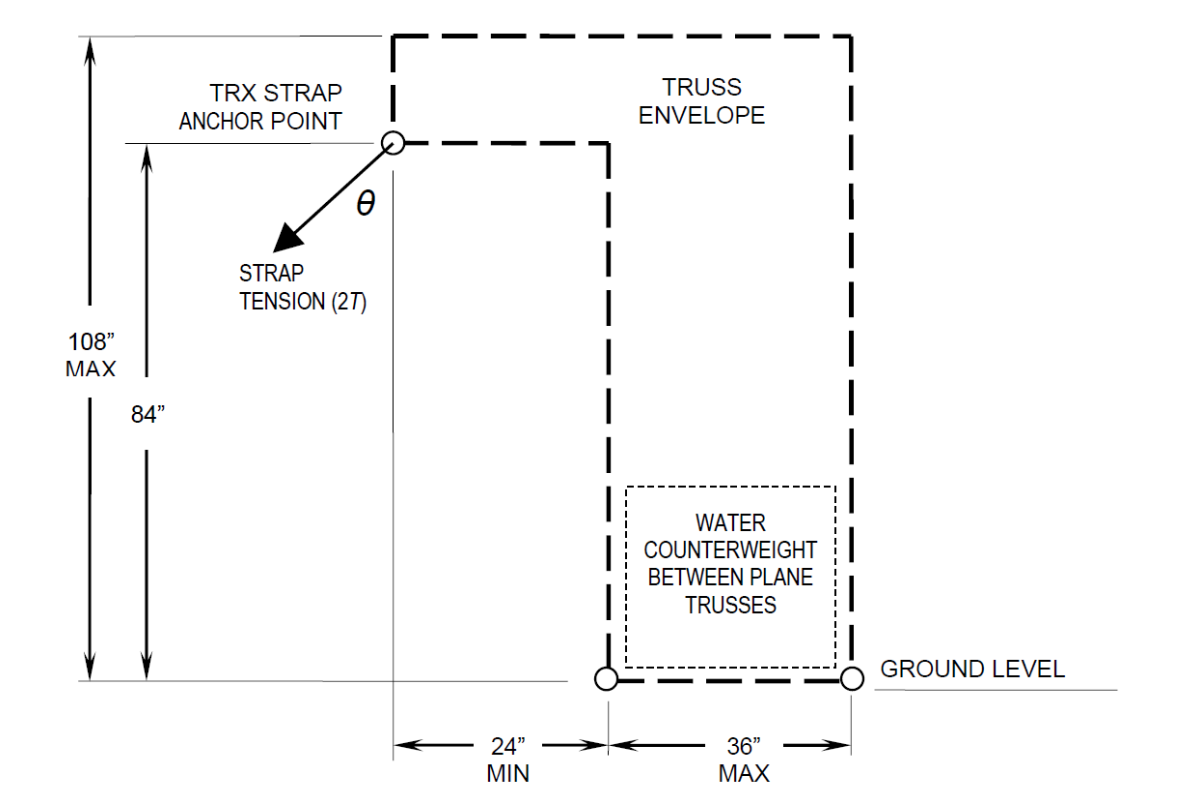
\includegraphics[width=7cm]{pr1.png}
    \caption{Specification Guidelines for Truss Frames}
\end{figure}
The truss members will be tubular aluminum with a maximum length $48$ inches, will not exceed ratings of $2800 lb$ in Tension, and $700 lb$ in Compression. The factor of safety for these values will be determined. Finally, the overall dimensions of the truss will be within the specified truss envelope as drawn in the figure above.\
For the water tank that rests within the truss envelope, the volume of water required for the stability of the two anchor points and the corresponding dimensions for the water tank are to be determined. The total length of the truss members are required, the volume of the water tank are to be determined in a minimized fashion. The water weight is equally distributed and applied to the two joints at ground level.\
The two planar trusses are attached with cross braces and the bottom braces to the anchoring points will support the plastic water tank that anchors the entire structure. The truss members will snap into specially designed joints that can be modeled as truss pin joints. The design of these joints to the point of further investigation is not required and goes beyond the scope of this design proposal, therefore the focus will be on the design of the truss.\
\chapter{Solution Procedure}
First, the outline of the tension at angles for each member should be clarified to the specification, which was specified in the previous definition. Therefore, we understand that a single side is symmetrical to the other frame and that it will be $36$ inches apart connected by the cross braces as specified. Now, the given data of the tank is what must be determined as it is not given. As one of the driving problems of the suspension system is leveraging one's weight against the counterweight, therefore the weight of the water counterweight must also equal the weight sustained by the load at the anchor where the TRX strap connects. Given the conventional water density $ \rho = 0.997 \frac{g}{cm^3 }$ and the constant of gravity at $ g = 9.81 \frac{m}{ s^2 }$ then the equivalent volume of the tank is equal to the load specification on the TRX strap as calculated below. Our assumptions are given as $ \Sigma M_A = 0, B_y = 0, \Sigma F_x = 0, \Sigma F_y = 0, W = f(T) $ and that the weight of the water is equally distributed and applied to the two joints at ground level.
$$(T \cos(45)) (h) + (T \sin(45)) (l) - A_{x,y}(\frac{W}{2}) + B_{y}(l)  \longrightarrow (150 \cos(45 )) (24 in) + (150 \sin(45)) (84 in) - (\frac{18W}{2}) + (0)(36) $$ 
$$ = 8100\sqrt{2} -9x = 0; x = 900 \sqrt{2} = 1272.8 $$
The force of $A$ is trivially found as the $A_x = 75 \sqrt{2}= 106.1, A_y =  \sum(A_x + A_y + B_y -  \frac{1272.8}{2}) = 742.46 = 742.5$ lb-f which is converted to $6602$ Newtons for the entire structure. The required volume is now calculated with the following equation: $V = \frac{6602 N}{0.997 (\frac{g}{m^3}) \cdot 9.81} = 0.675 m^3$
Volume tank dimensions cannot exceed $36$ inches, thus when we take the maximum reaction of the two joints at ground level, there is a rounded almost square tank of water thus the diameter and height do not exceed the previously defined values giving us a base Volume of water of for the vertical rounded square tank with $ 231.27 $ cm , taking our equation to find the maximum height to be at most $91$ inches.  
In calculating the given tension/compression of each section of truss, the determination of safety becomes apparent through the results in theory. 
\section{Design and Analysis Process}
The method of determining forces in the members of the truss is method of joints, where we look at the equilibrium of the pin at the joints. Since the forces are concurrent at the pin, there is no moment equation and only two equations for equilibrium.
$$ \sum F_{x} = 0$$
$$\sum F_{y} = 0 $$
To start, we analyze at a point where one known load and at most two unknown forces are there. The weight of each member is divided into two halves and that is supported by each pin. To an extent, this method is directly inspired by the design and consequently influences the analysis phase. \\
As shown in the detailed freebody diagrams, each joint is considered as method of joints to solve the statically determinate entire structure. For trusses, wethe planar trusses formulas for quick checking a structure is not indeterminate, or improperly restrained, such that all unknowns could be found using the techniques in statics for writing equilibrium equations. \\
By the nature of writing and solving equilibrium equations iff a solution exists, the structure is determinant.\\
Method of joints requires subsequently requires determining the external reactions then the internal forces in each of the members to evaluate by tension or compression.\\
Therefore, we will be able to solve through each joint by freebody diagram. Then, to solve the joints, the construction of a system of equations to find the independent equations and solve the unknowns is the best and mathematically correct method. What is also true for the trusses designed is that there are joints that connect members aligned along the same line, therefore the zero-force members will be noted on the free-body diagram as well. \\
\chapter{Conceptual Designs}
Each design concept proposed is tested to verify that each structure design concept is statically determinant and stable. To classify the truss as determinate, it requires an examination at the joining of the simple trusses in the proposed designs for the structures. Therefore, the following metric is used to determine the truss is determinate or not: $2n = m + r$ where $m$ stands for members, $r$ stands for reactions, and $n$ represents joints. Now the necessary conditions for evaluating statical determinancy is not dependent on insufficient conditions to prove the relationship by contradiction, however if the truss satisfies the defined relation, it may not be determinate. This is why it is careful to understand that determinate trusses satisfy the above relation but require further clarification. 
\section{Concept 1}
This design concept has been checked to be statically determinant and stable by the following metrics: \medskip
\begin{center}
\begin{tabular}{|r|l|c}
\cline{1-2}
\textbf{joints} & $9$ & \begin{tabular}[c]{@{}c@{}}$m + 3 = 2j$\\ $15 + 3 = 2(9)$\end{tabular} \\ \cline{1-2}
\textbf{members} & $15$ & $18 = 18 $ \\ \cline{1-2}
\textbf{reactions} & $3$ & $2n \equiv m + r $ \\ \cline{1-2}
\end{tabular}
\end{center}
\medskip
Therefore,  $ 18 = 18 $ and LHS $\equiv$ RHS condition is satisfied thus it is true for this concept. 
\begin{figure}
\centering{\subsubsection{Sketch}}
\centering
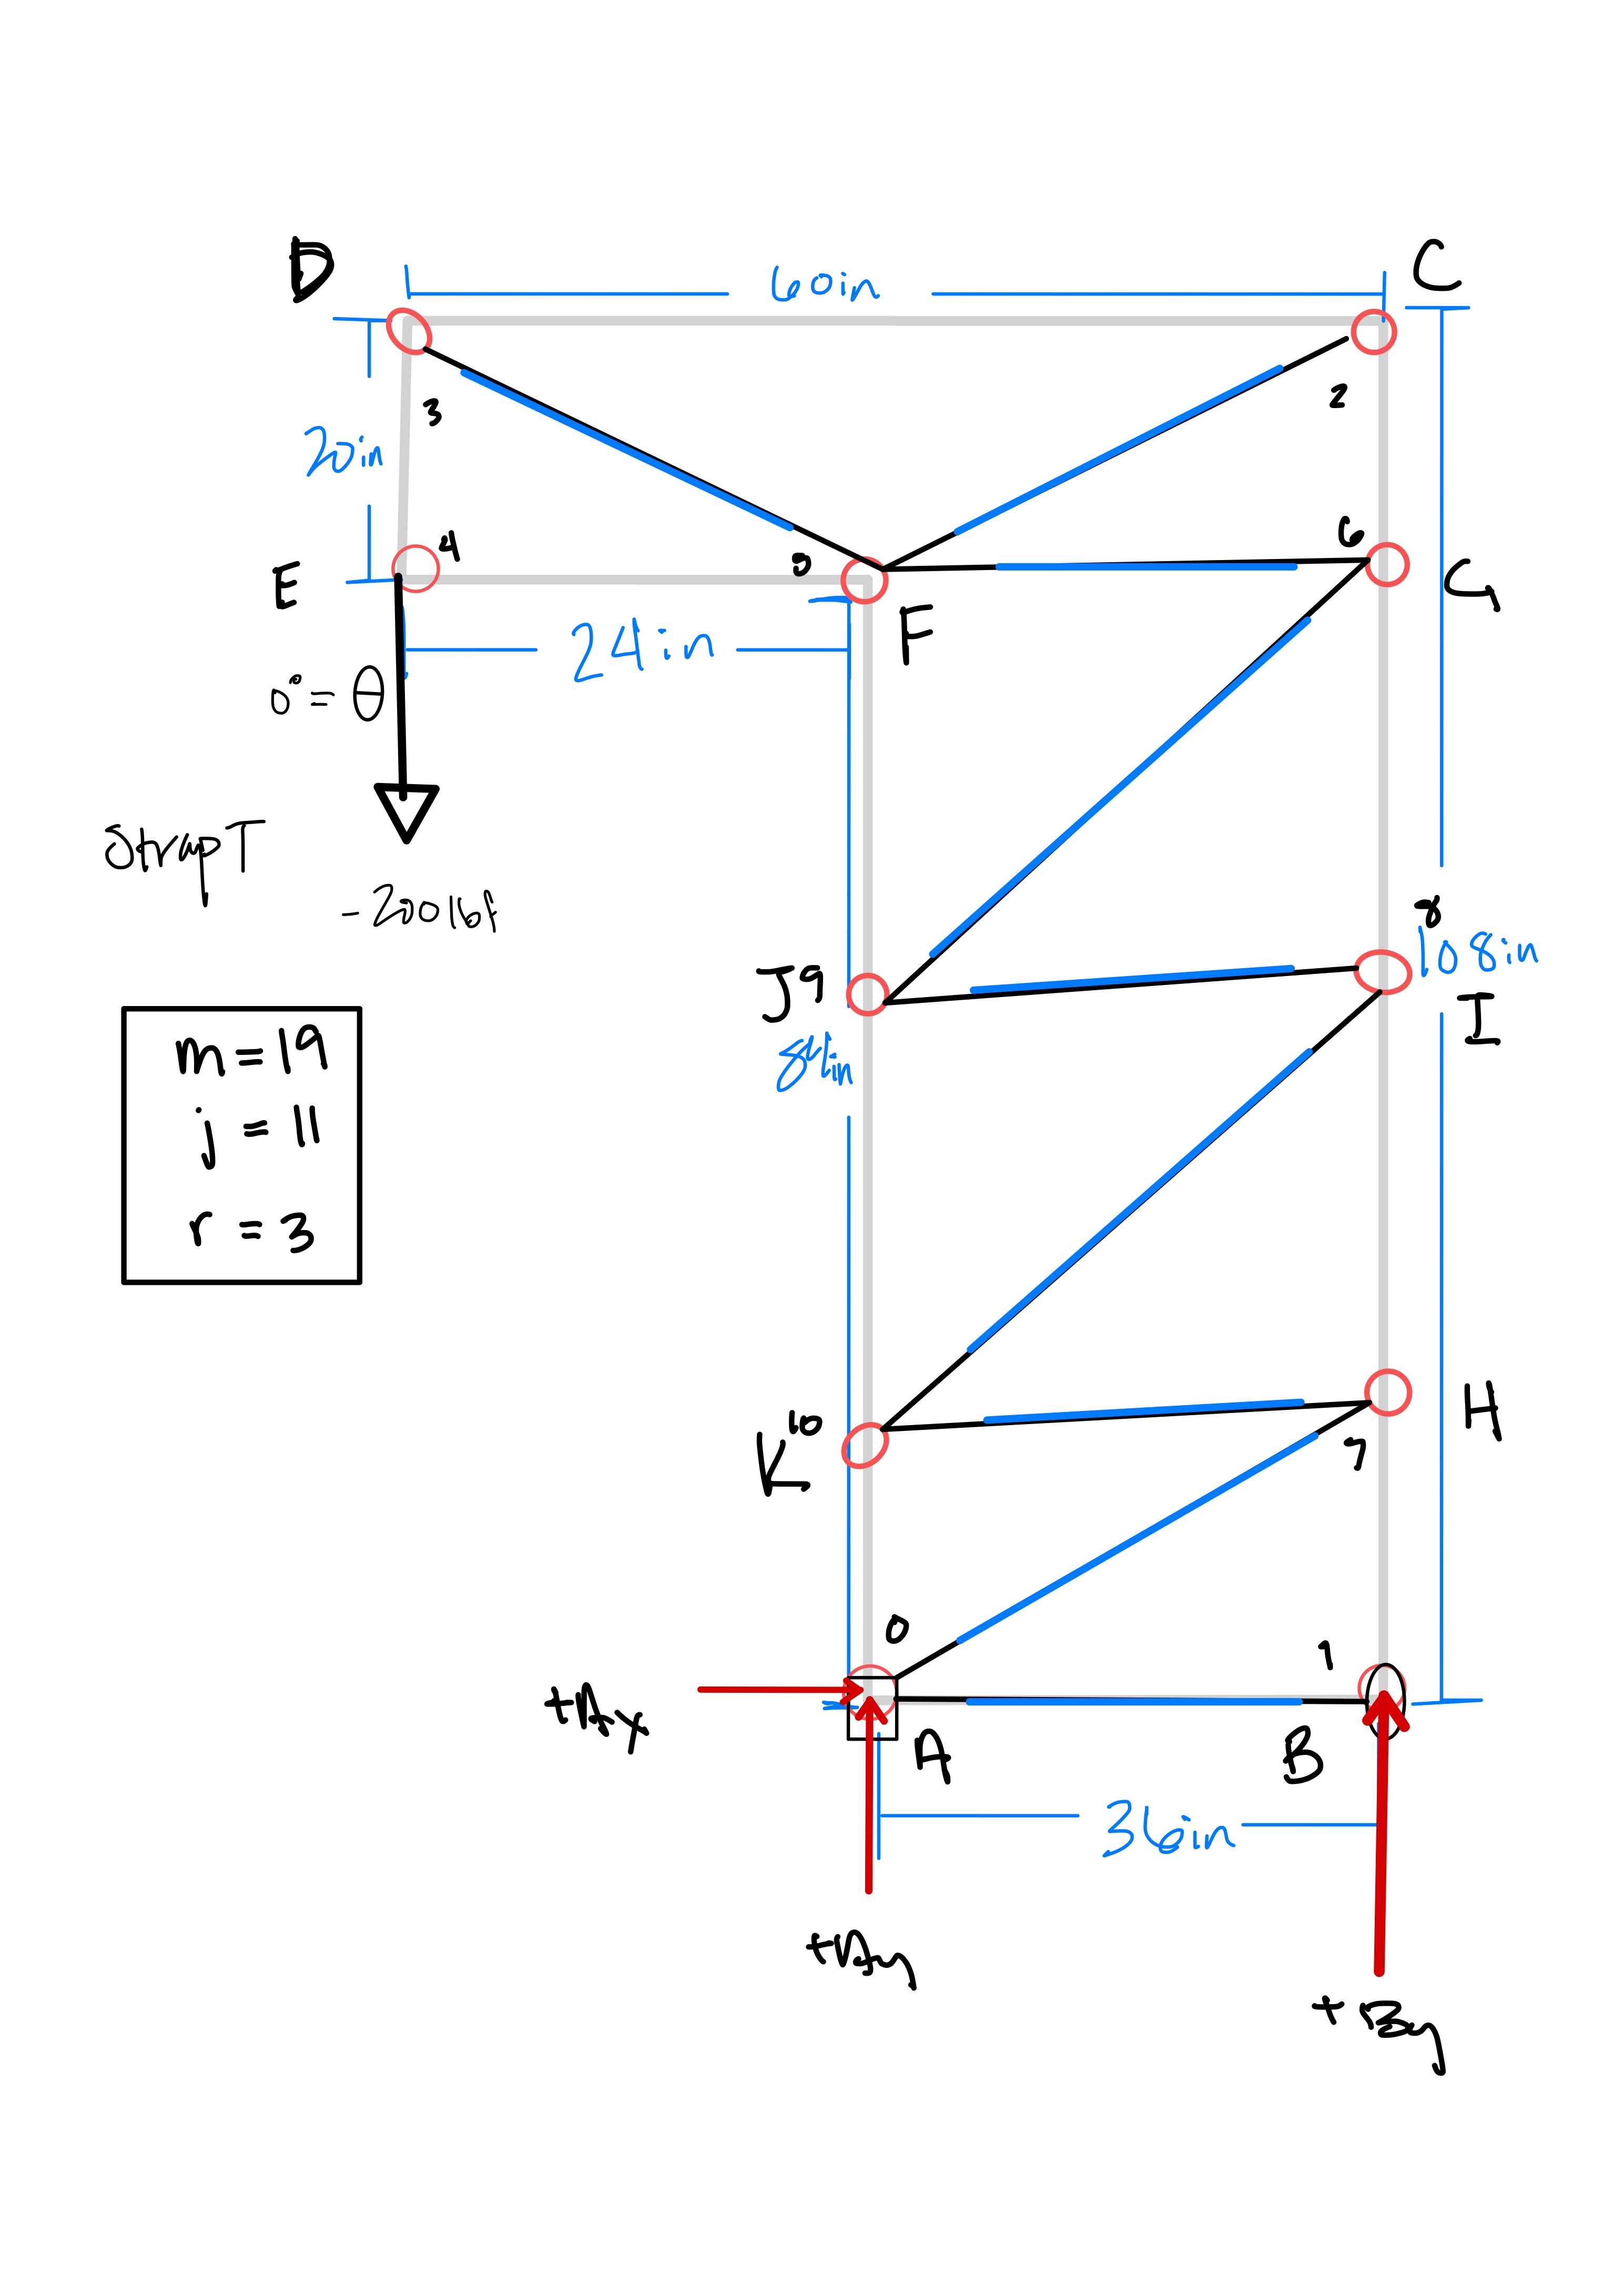
\includegraphics[width=\textwidth]{con2_lca.jpg}
\caption{Load Condition B at $\theta = 0$ degrees}
\end{figure}
\begin{figure}
\centering{\subsubsection{Sketch}}
\centering
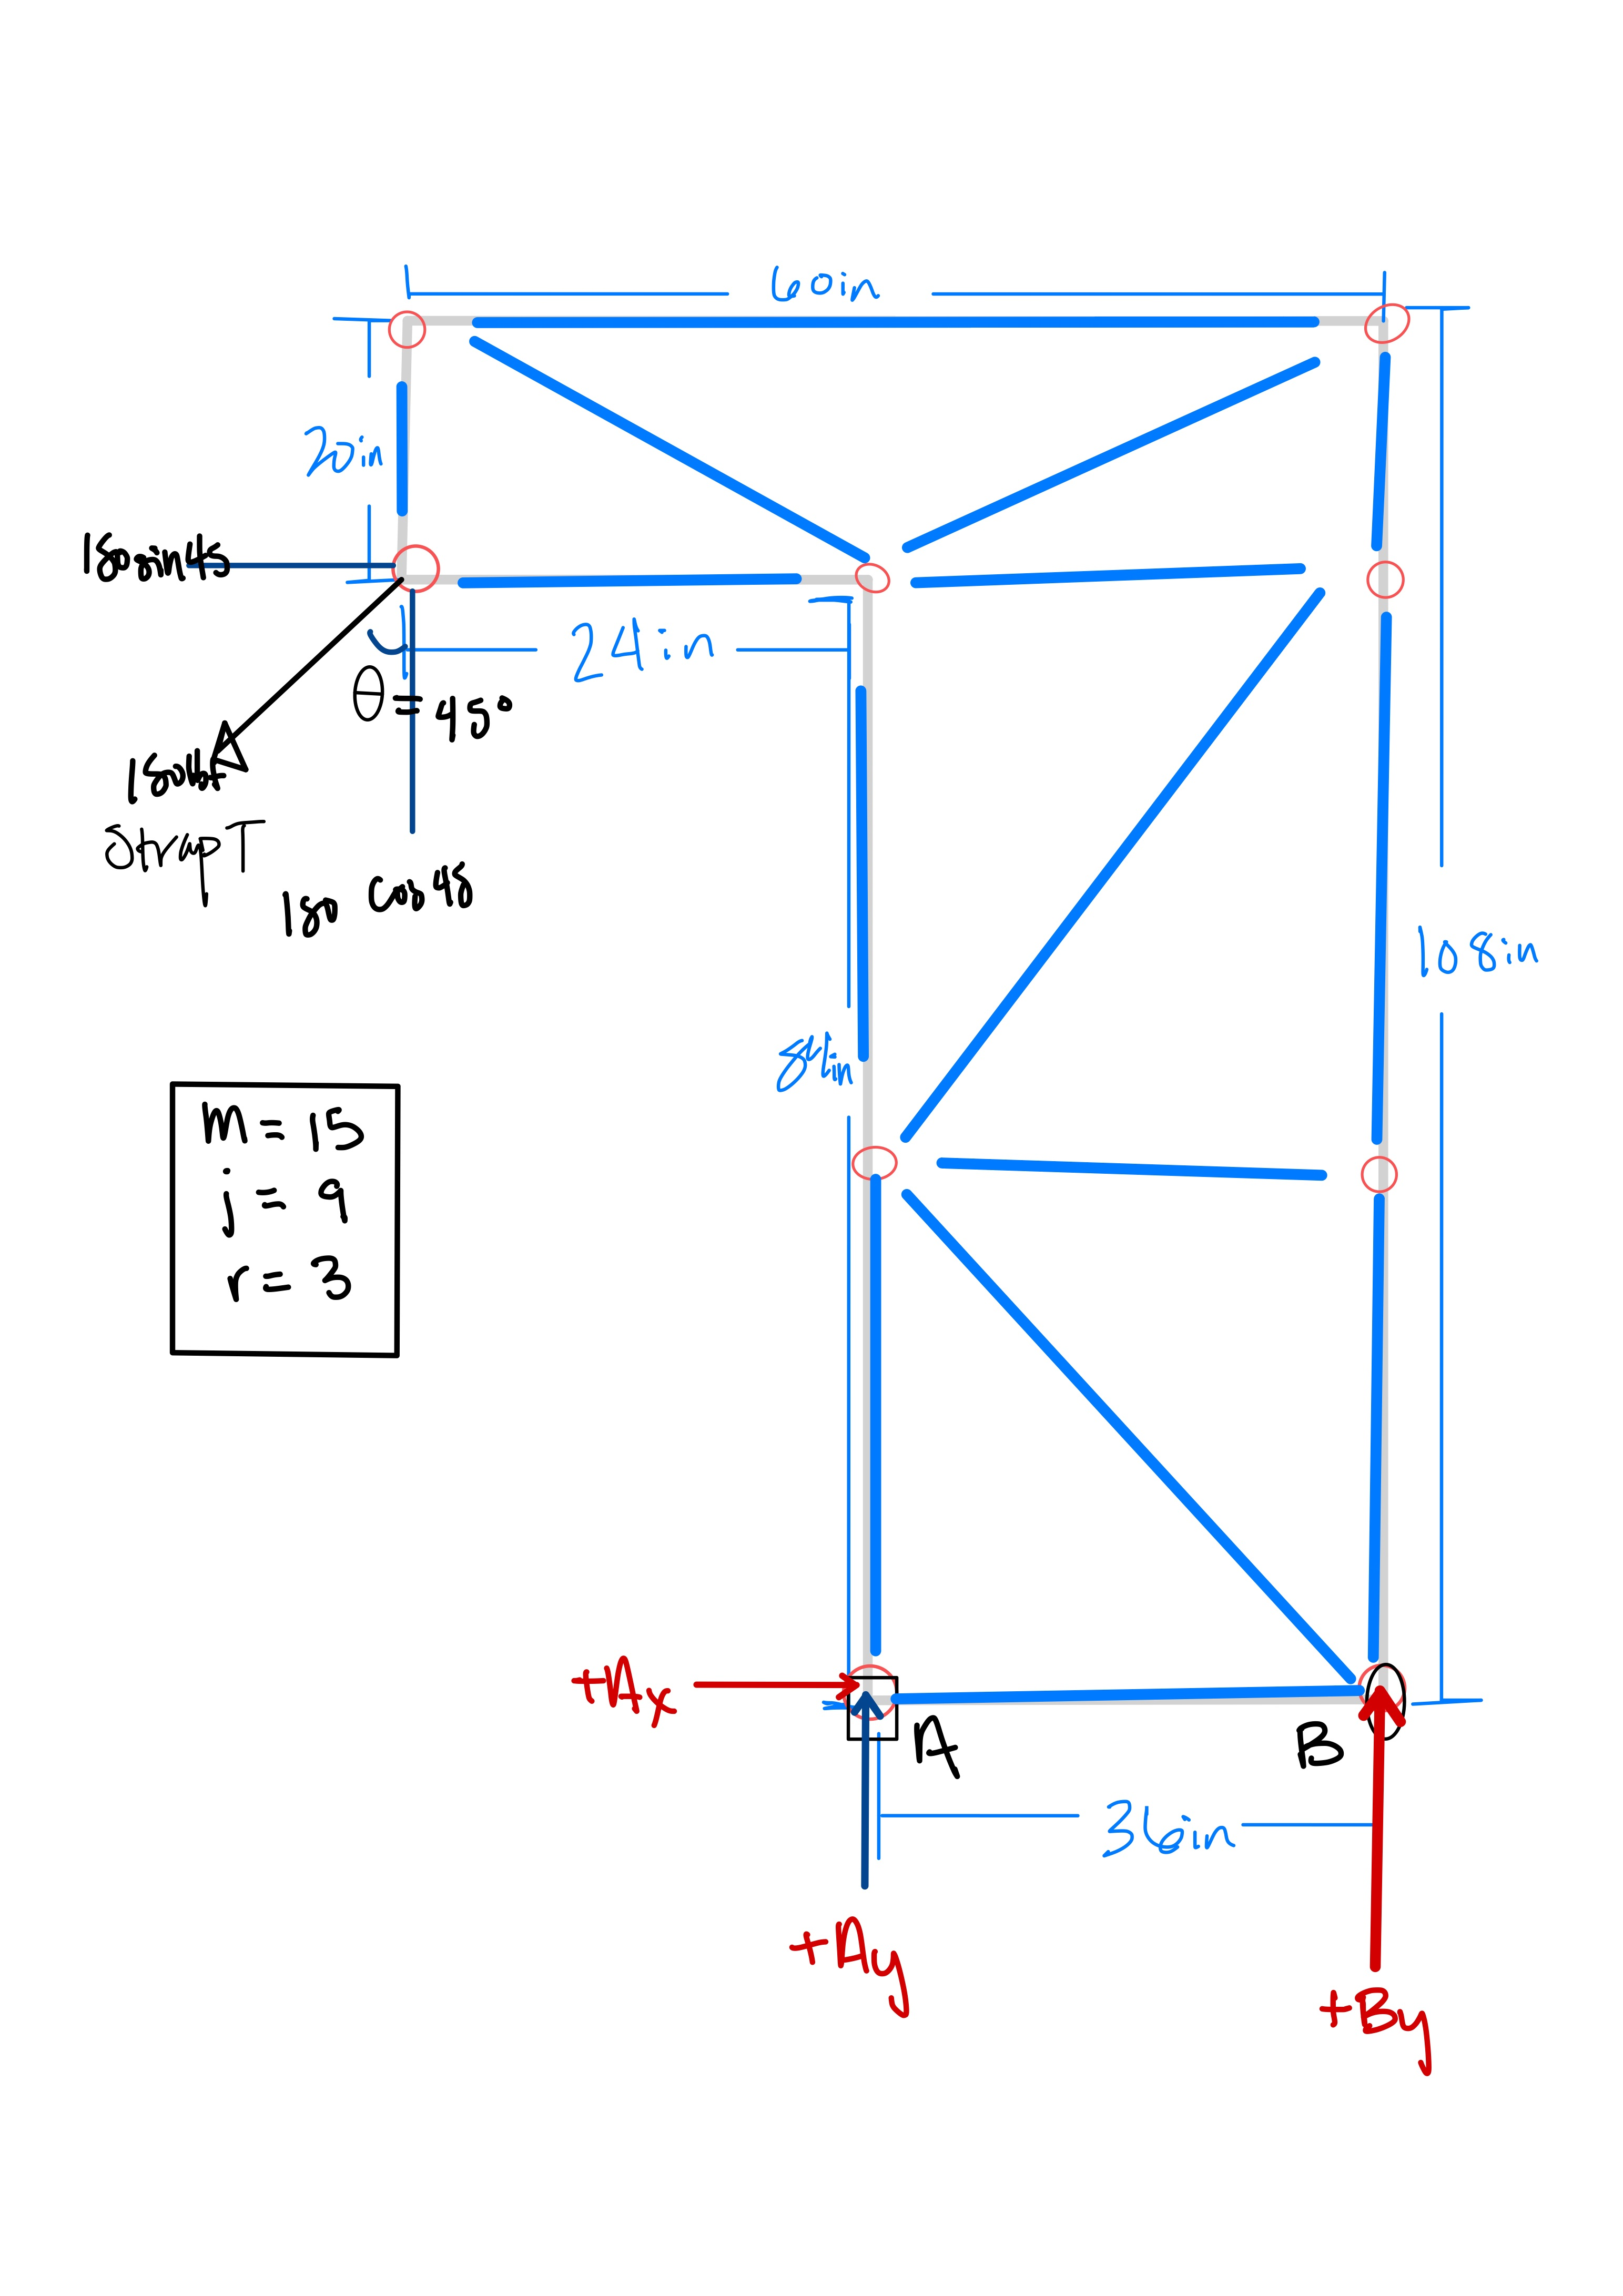
\includegraphics[width=\textwidth]{con1_lcb.jpg}
\caption{Load Condition B at $\theta = 45$ degrees}
\end{figure}
\section{Concept 2}
This design concept has been checked to be statically determinant and stable by the following metrics: 
\medskip
\begin{center}
\begin{tabular}{|r|l|c}
\cline{1-2}
\textbf{joints} & $11$ & \begin{tabular}[c]{@{}c@{}}$m + 3 = 2j$\\ $19 + 3 = 2(11)$\end{tabular} \\ \cline{1-2}
\textbf{members} & $19$ & $22 = 22 $ \\ \cline{1-2}
\textbf{reactions} & $3$ & $2n \equiv m + r $ \\ \cline{1-2}
\end{tabular}
\end{center}
\medskip
Therefore,  $ 22 = 22 $. The necessary conditions for statical determinancy have so far been passed. 

    \begin{figure}
\centering{\subsubsection{Sketch}}
    \centering
    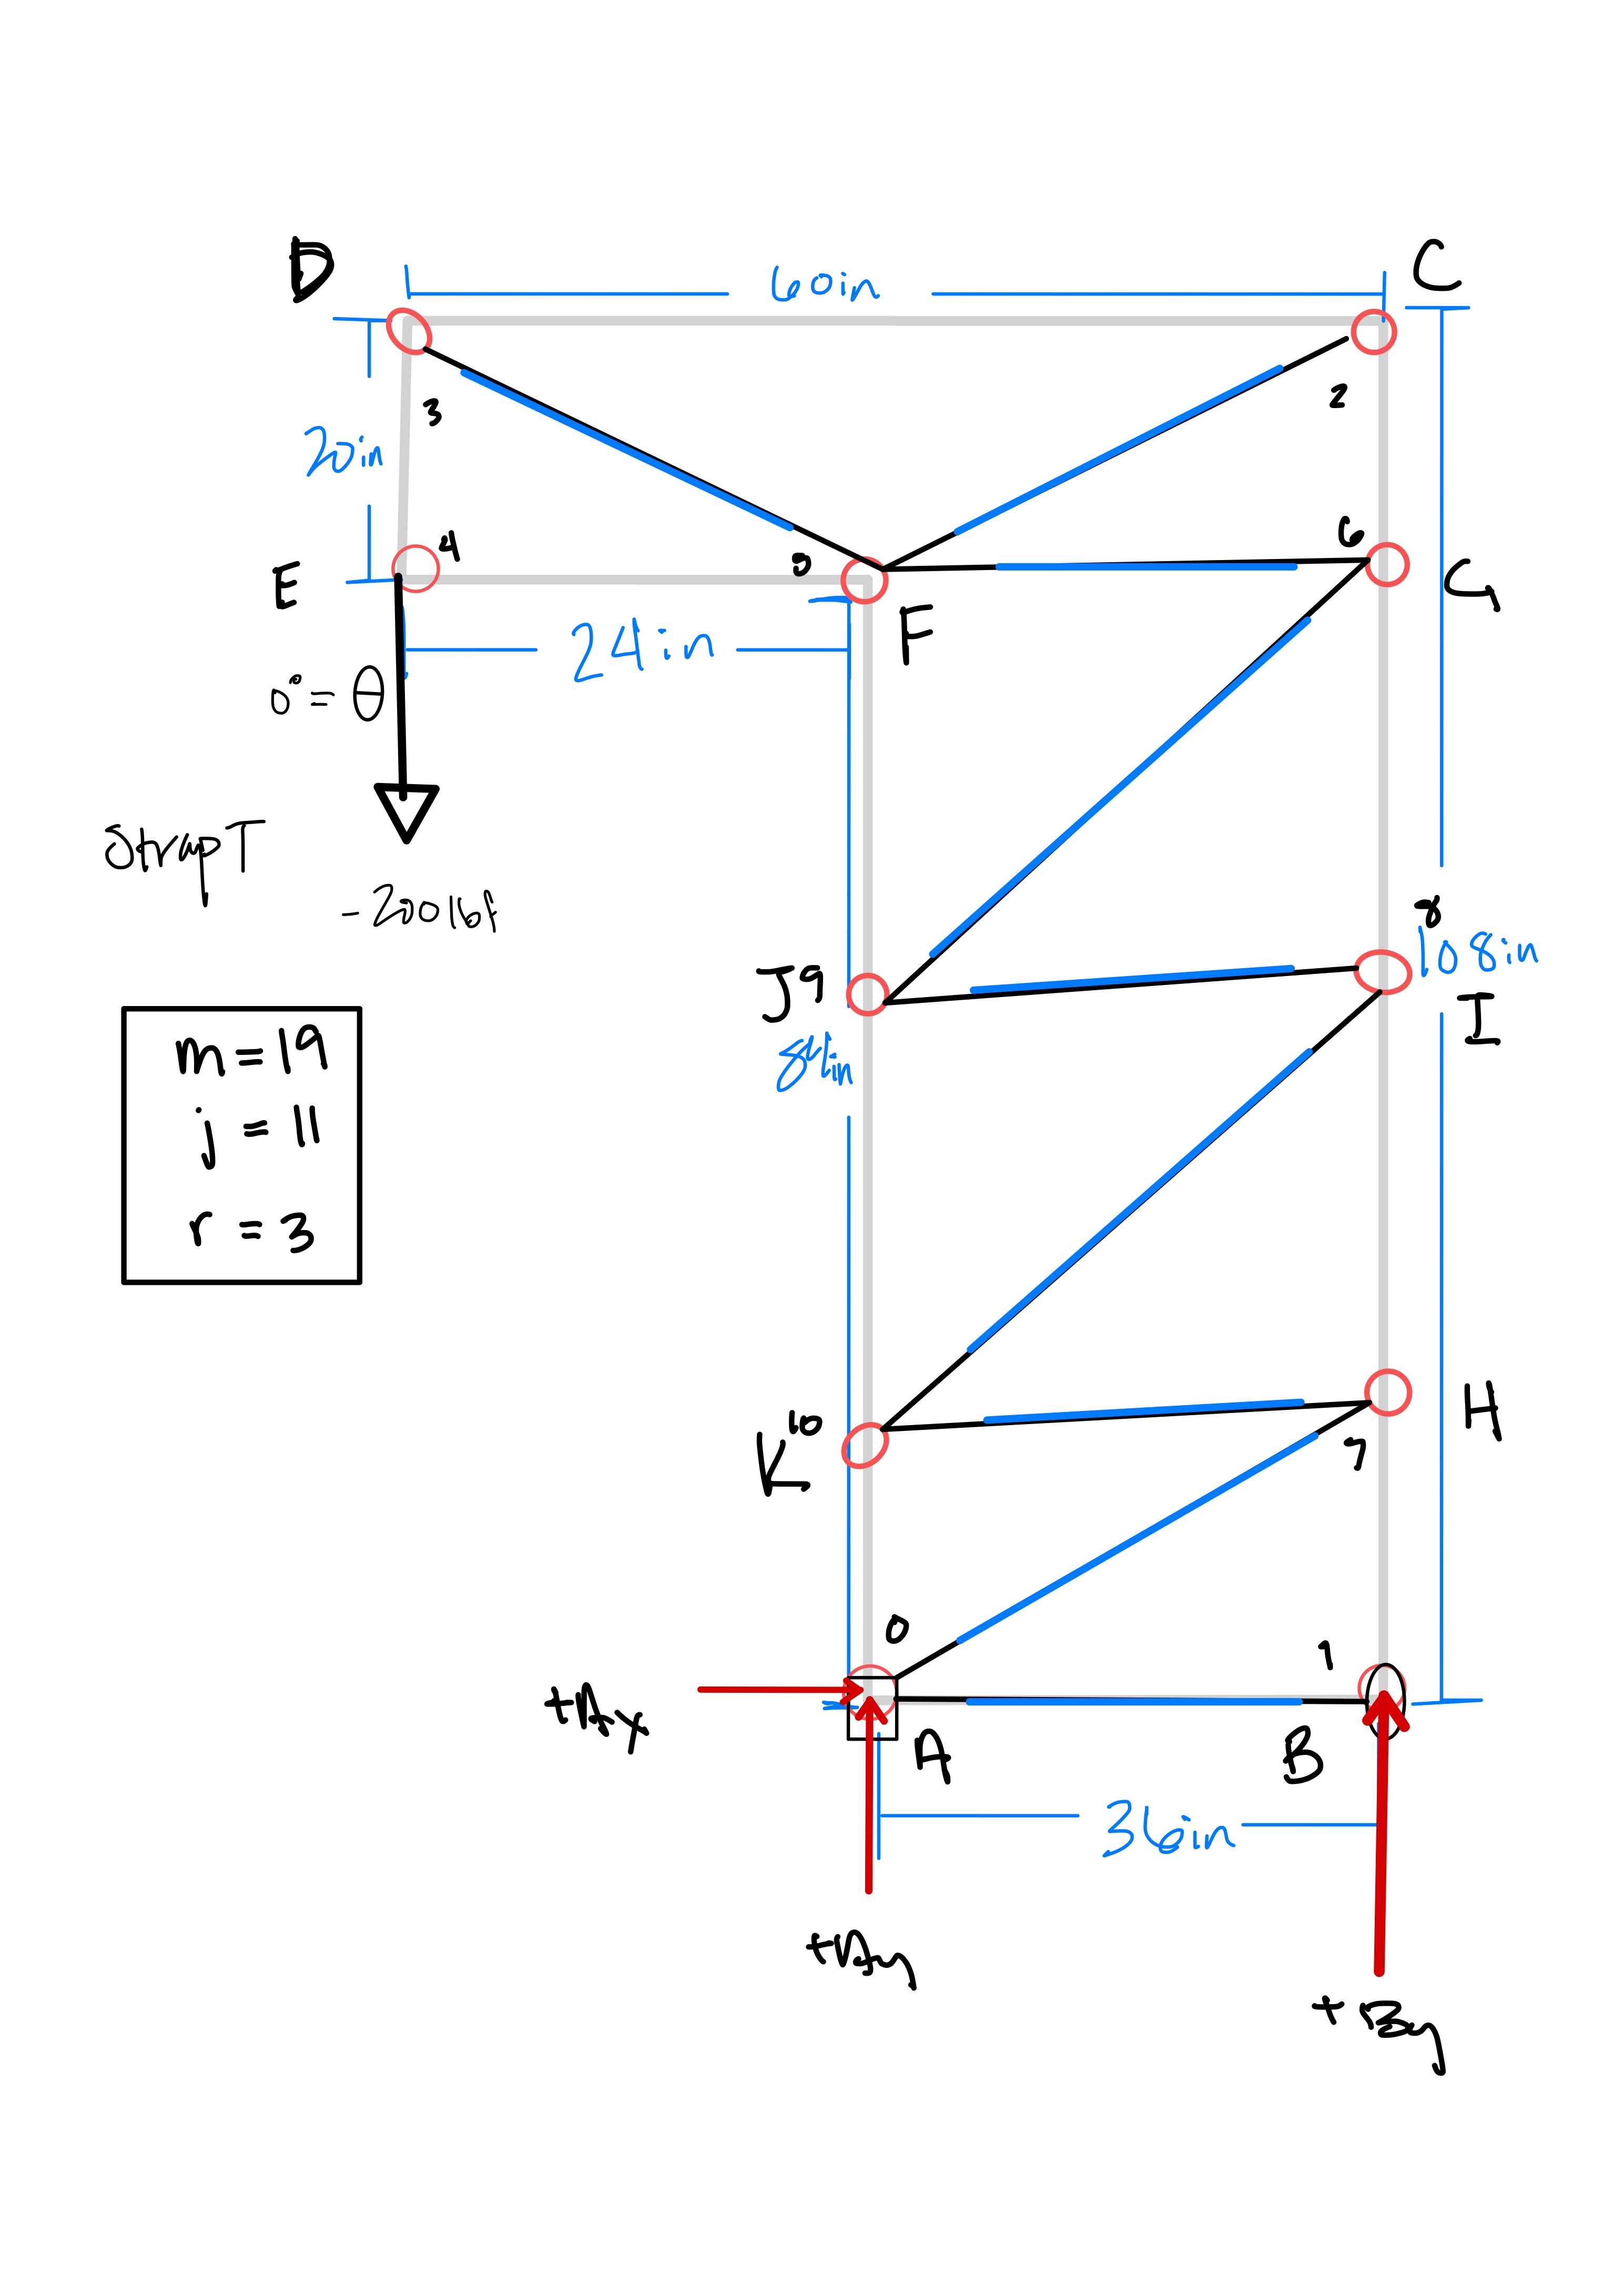
\includegraphics[width=\textwidth]{con2_lca.jpg}
    \caption{Load Condition A at $\theta = 0$ degrees}
\end{figure}
\begin{figure}
\centering{\subsubsection{Sketch}}
    \centering
    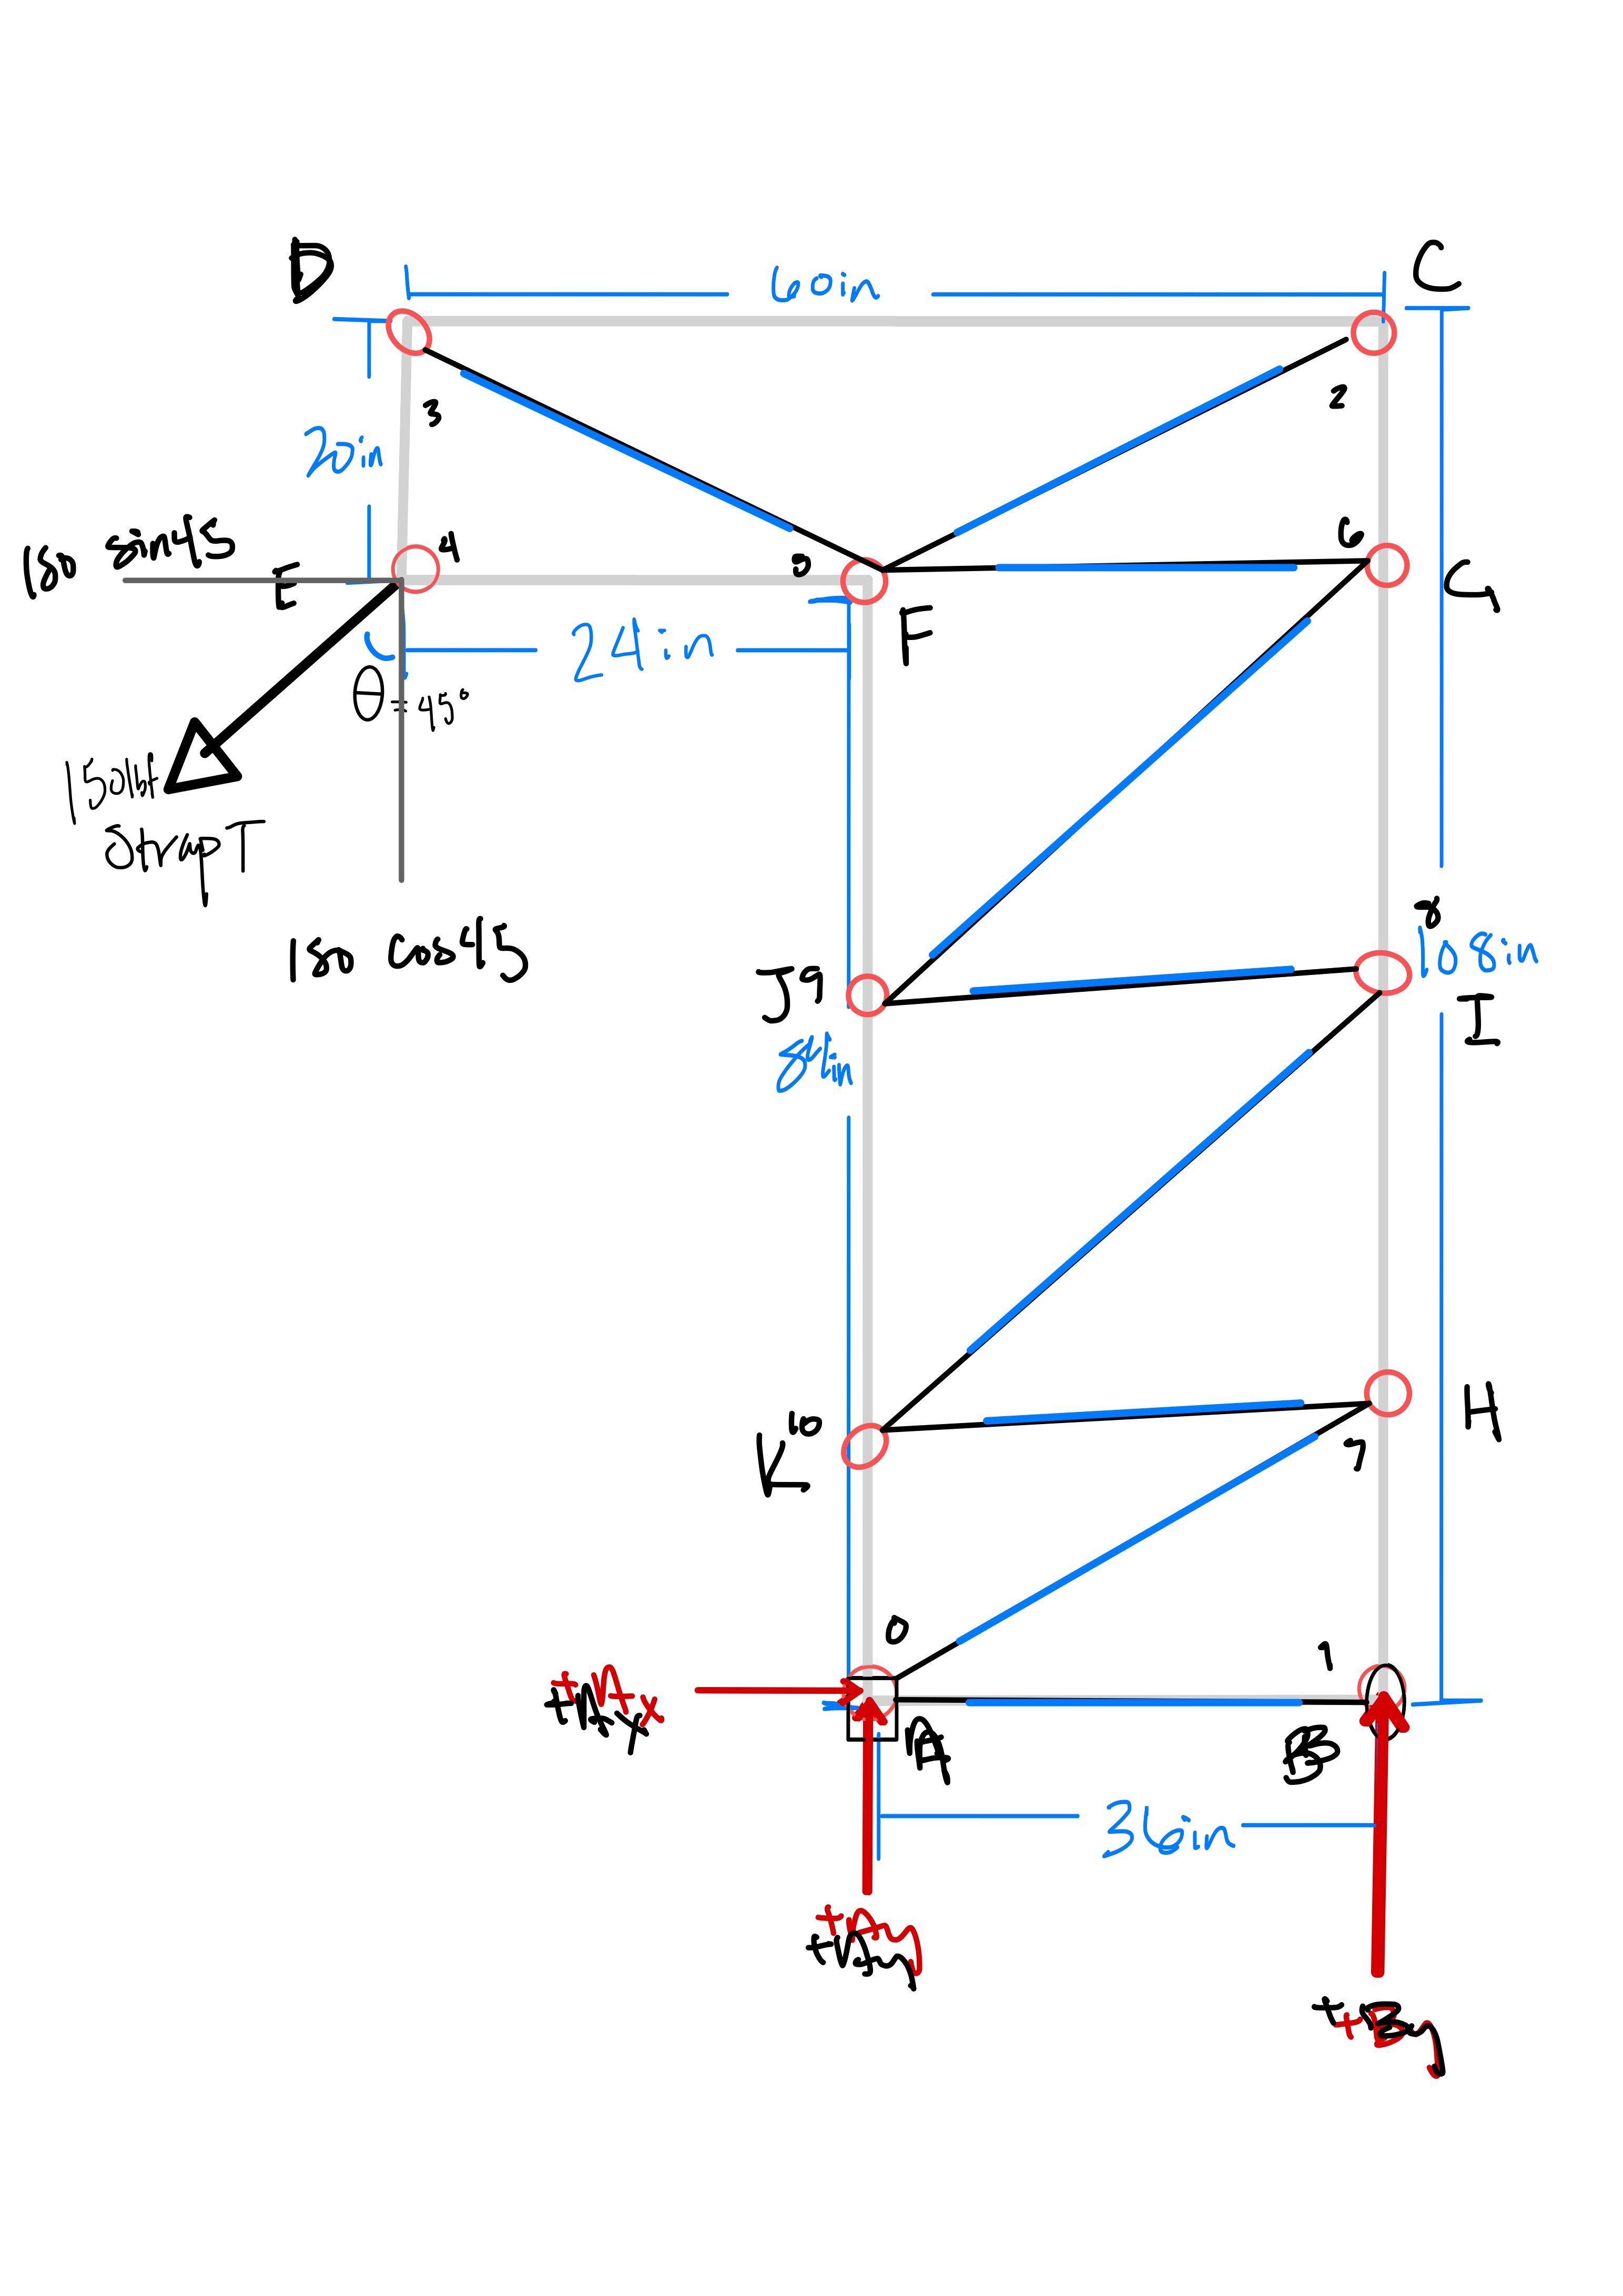
\includegraphics[width=\textwidth]{con2_lcb.jpg}
    \caption{Load Condition B at $\theta = 45$ degrees}
\end{figure}
\section{Concept 3}
This design concept has been checked to be statically determinant and stable by the following metrics:
\medskip
\begin{center}
\begin{tabular}{|r|l|c}
\cline{1-2}
\textbf{joints} & $10$ & \begin{tabular}[c]{@{}c@{}}$m + 3 = 2j$\\ $17 + 3 = 2(10)$\end{tabular} \\ \cline{1-2}
\textbf{members} & $17$ & $20 = 20 $ \\ \cline{1-2}
\textbf{reactions} & $3$ & $2n \equiv m + r $ \\ \cline{1-2}
\end{tabular}
\end{center}
\medskip
Therefore,  $ 20 = 20 $, which is true. The structure is stable and statically determinant (otherwise the unknowns would be too great to solve the structure evenly as well).
\begin{figure}
\centering{\subsubsection{Sketch}}
\centering
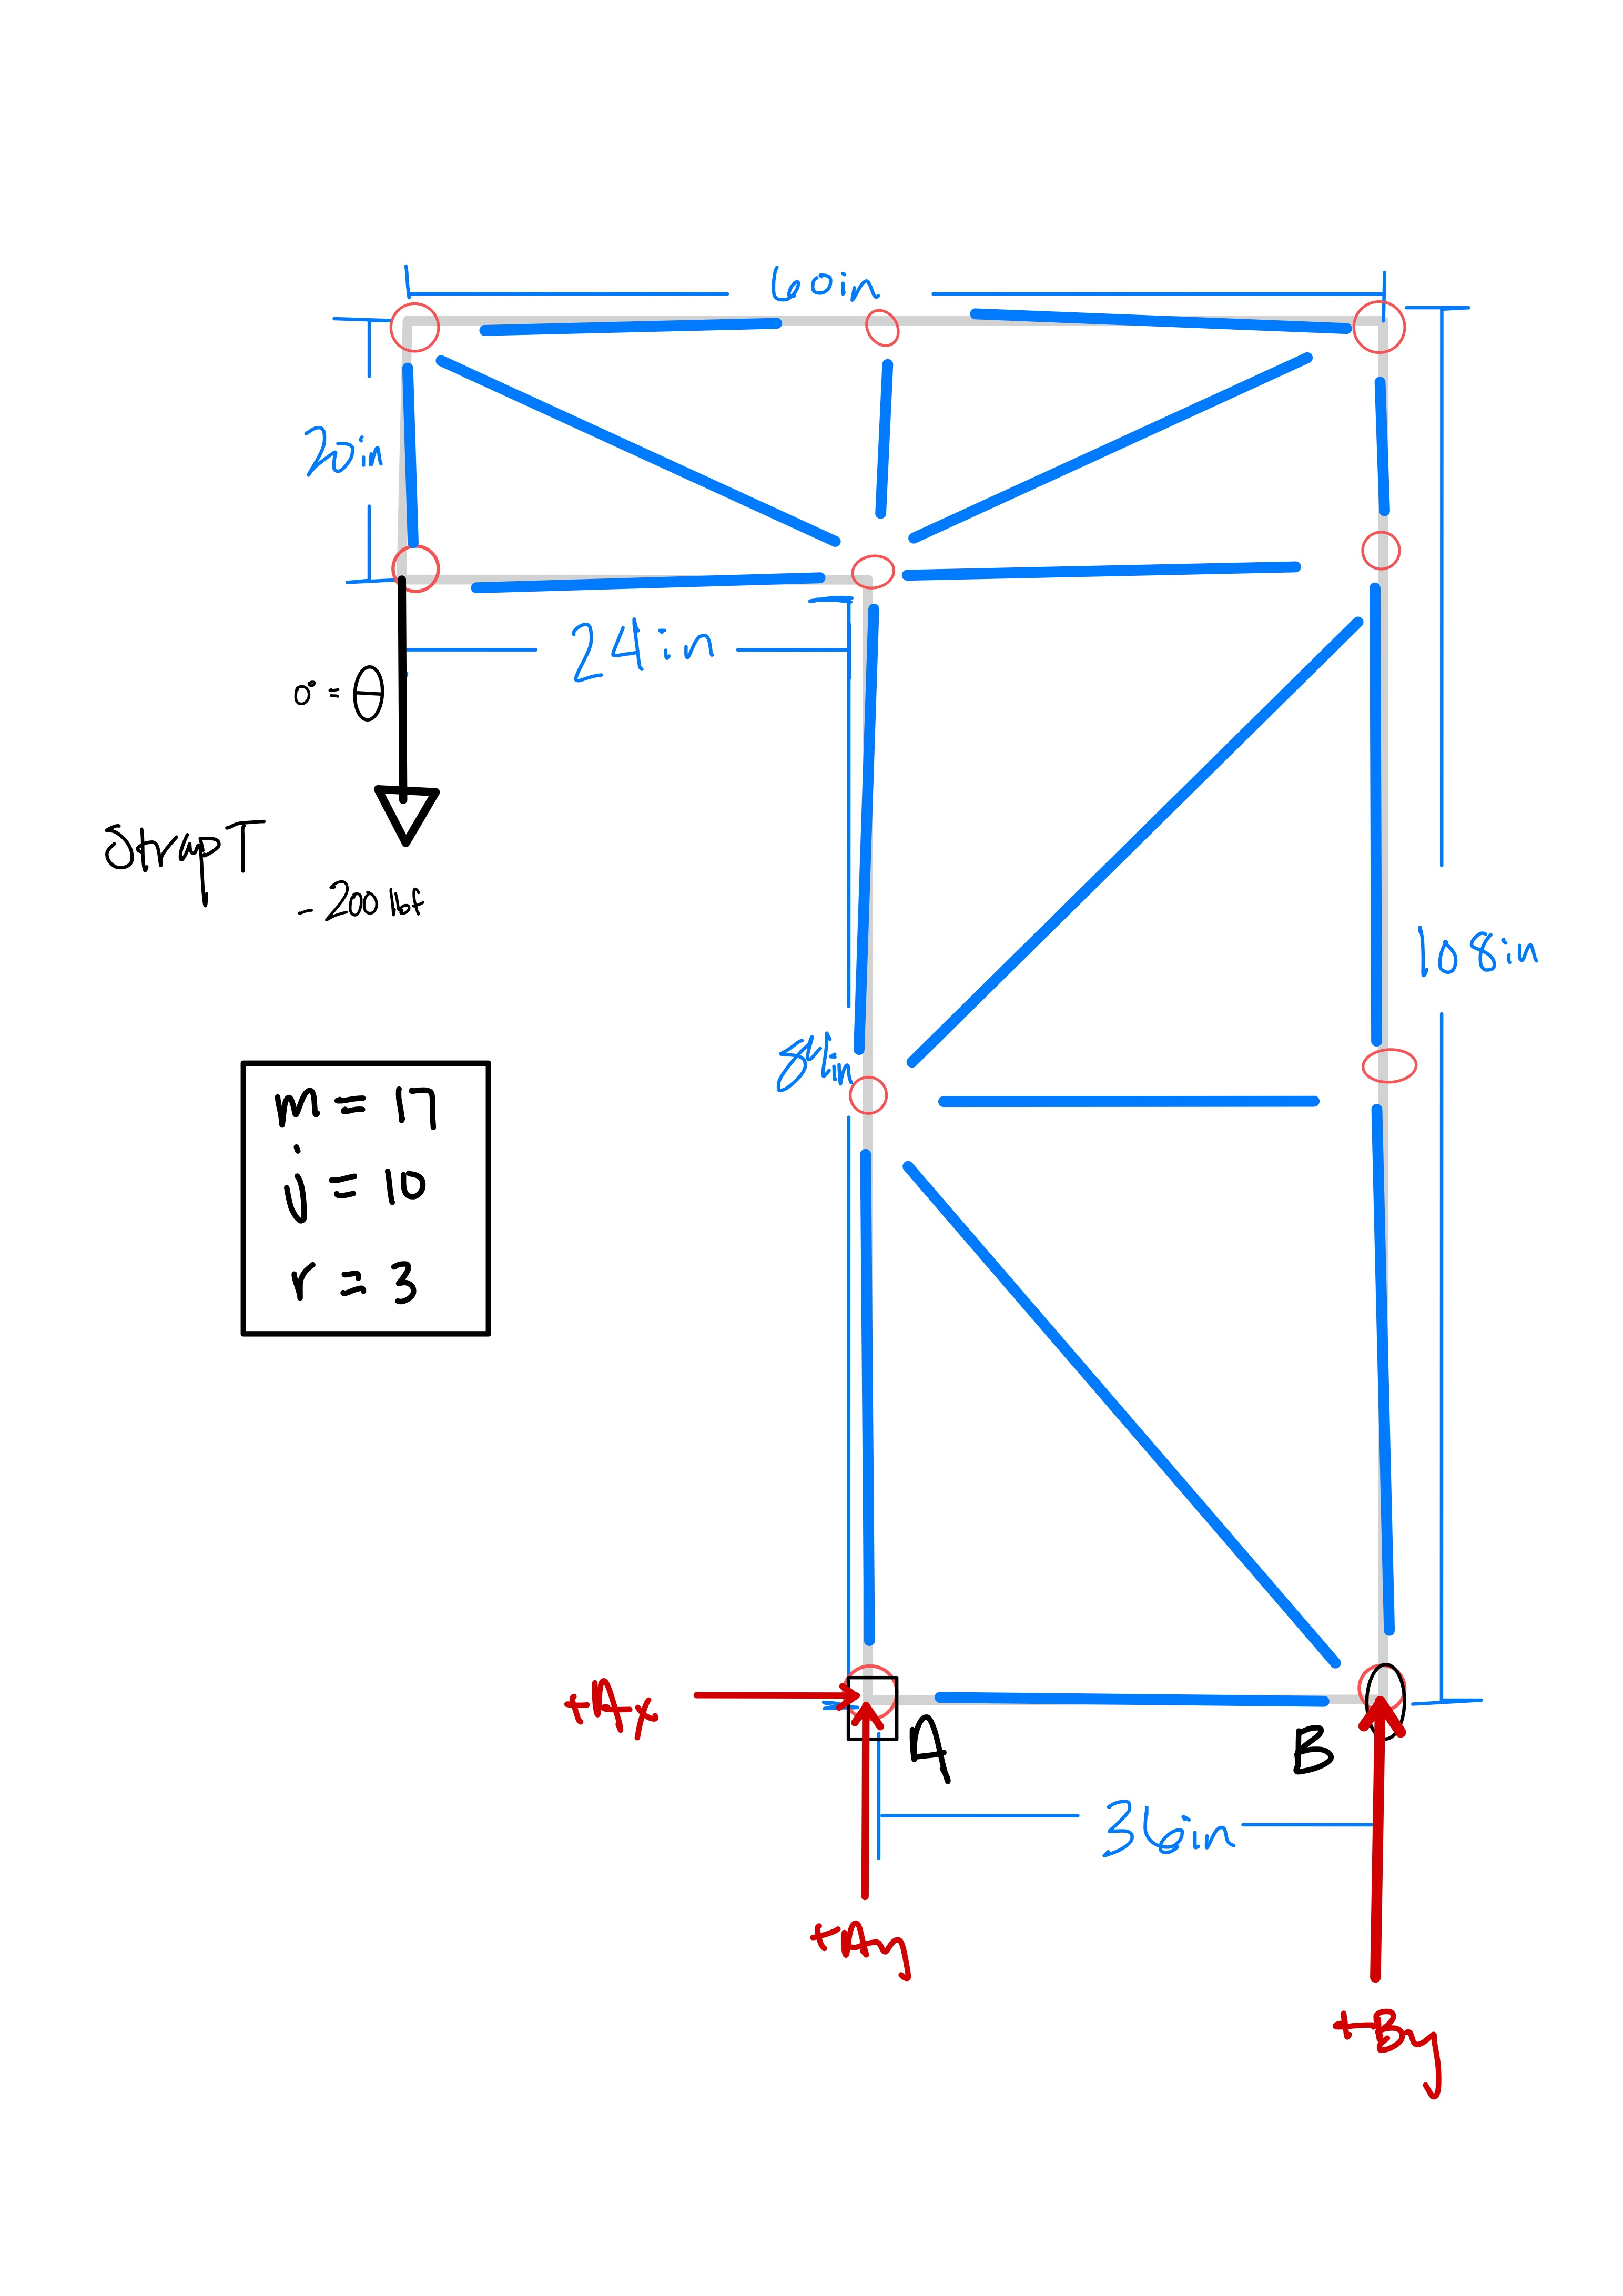
\includegraphics[width=\textwidth]{con3_lca.jpg}
\caption{Load Condition B at $\theta = 0$ degrees}
\end{figure}
\begin{figure}
\centering{\subsubsection{Sketch}}
\centering
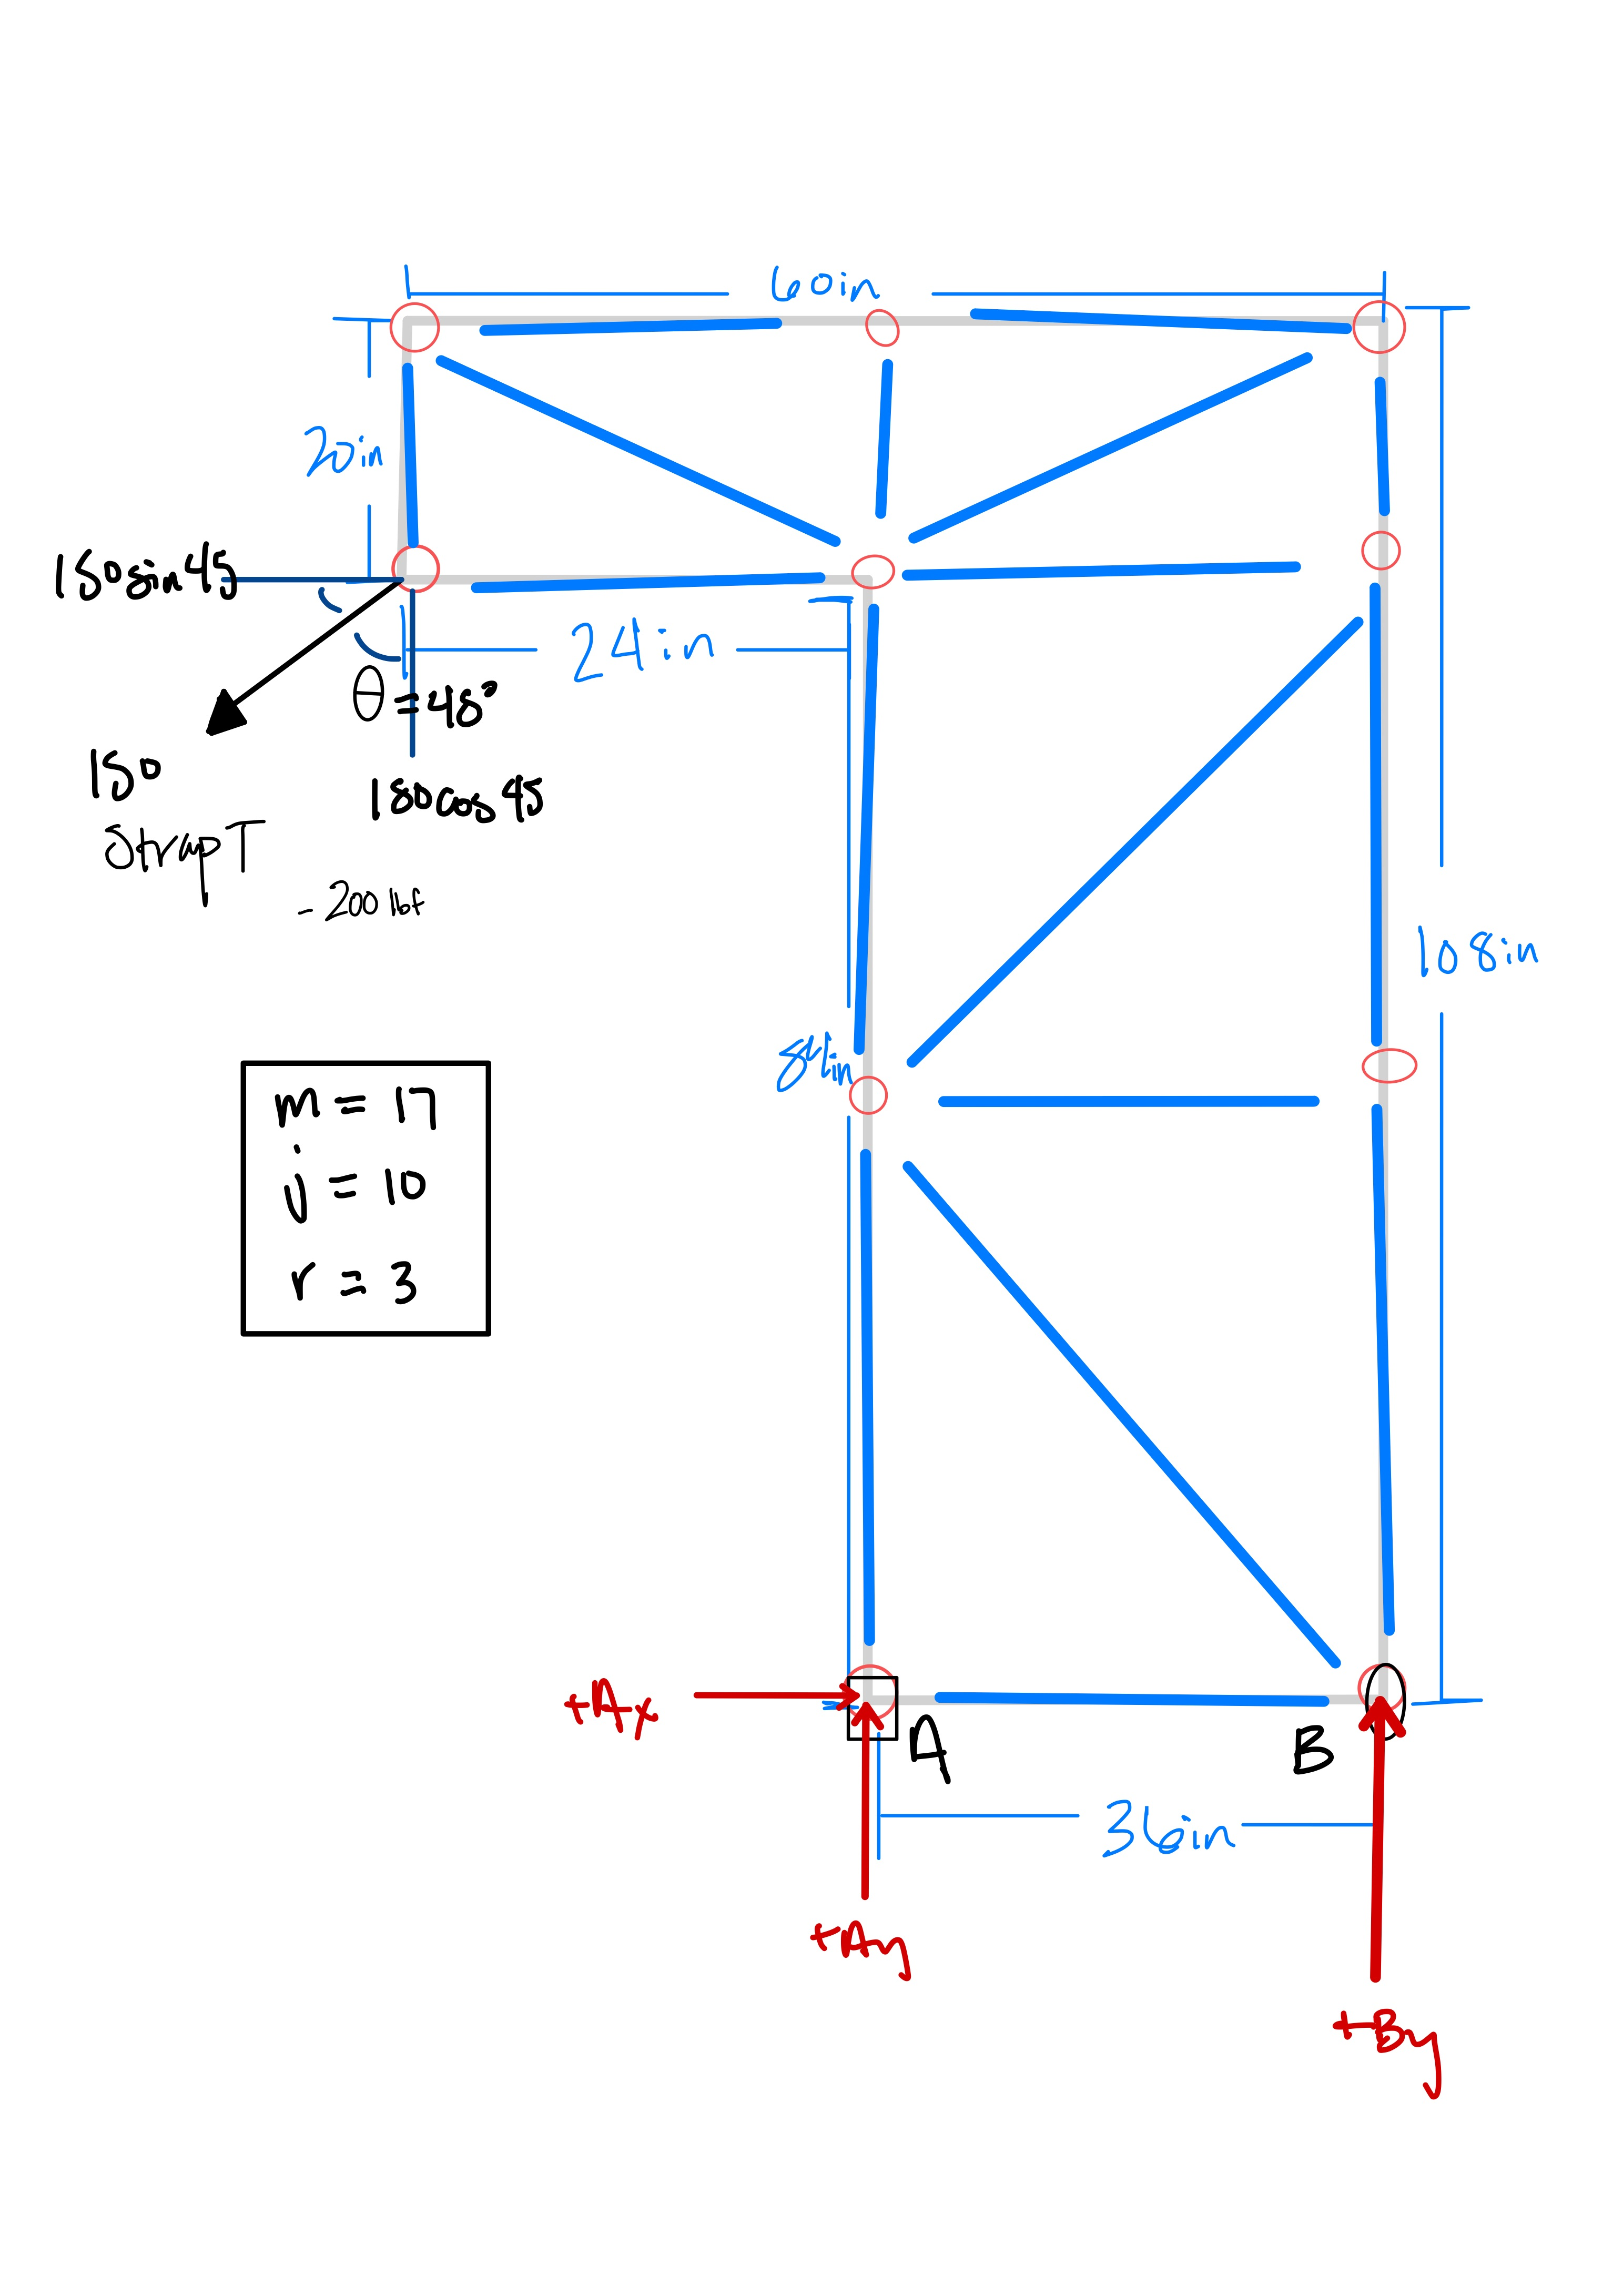
\includegraphics[width=\textwidth]{con3_lcb.jpg}
\caption{Load Condition B at $\theta = 45$ degrees}
\end{figure}
\chapter{Analysis of the Proposed Designs}
\section{Results}
	The truss analyzed in each subsection involves determining the external and internal forces/reactions of each member to determine Tension or Compression. Previously, the external reactions were defined but are noted here () for reference.
$$ \Sigma F_x = 0 \longrightarrow $$
$$ \Sigma F_y = 0 \longrightarrow $$ $$ \Sigma M_A = 0 \longrightarrow $$
    
    The internal forces are simplified but sketched the complete free body diagram, the method of solving used is method of joints. Table for each concept listing the length and the calculated force in each members + the total length of the truss members required for each concept.

\subsection{Concept 1: Load Condition A}
	At $ \theta = 0 $ degrees, then we can solve for the following: $\frac{w}{2} = \frac{400}{2} = -200 $ lb-f. For each joint we require a free body diagram calculating each joint by method of joints.
        \subsubsection{External reactions}
$ A_x = 0 $ lbf, $A_y = 333$ lb-f. $ B_y = -133$ lbf.
\subsubsection{Internal Forces (Compression/Tension)}
\begin{figure}
\centering
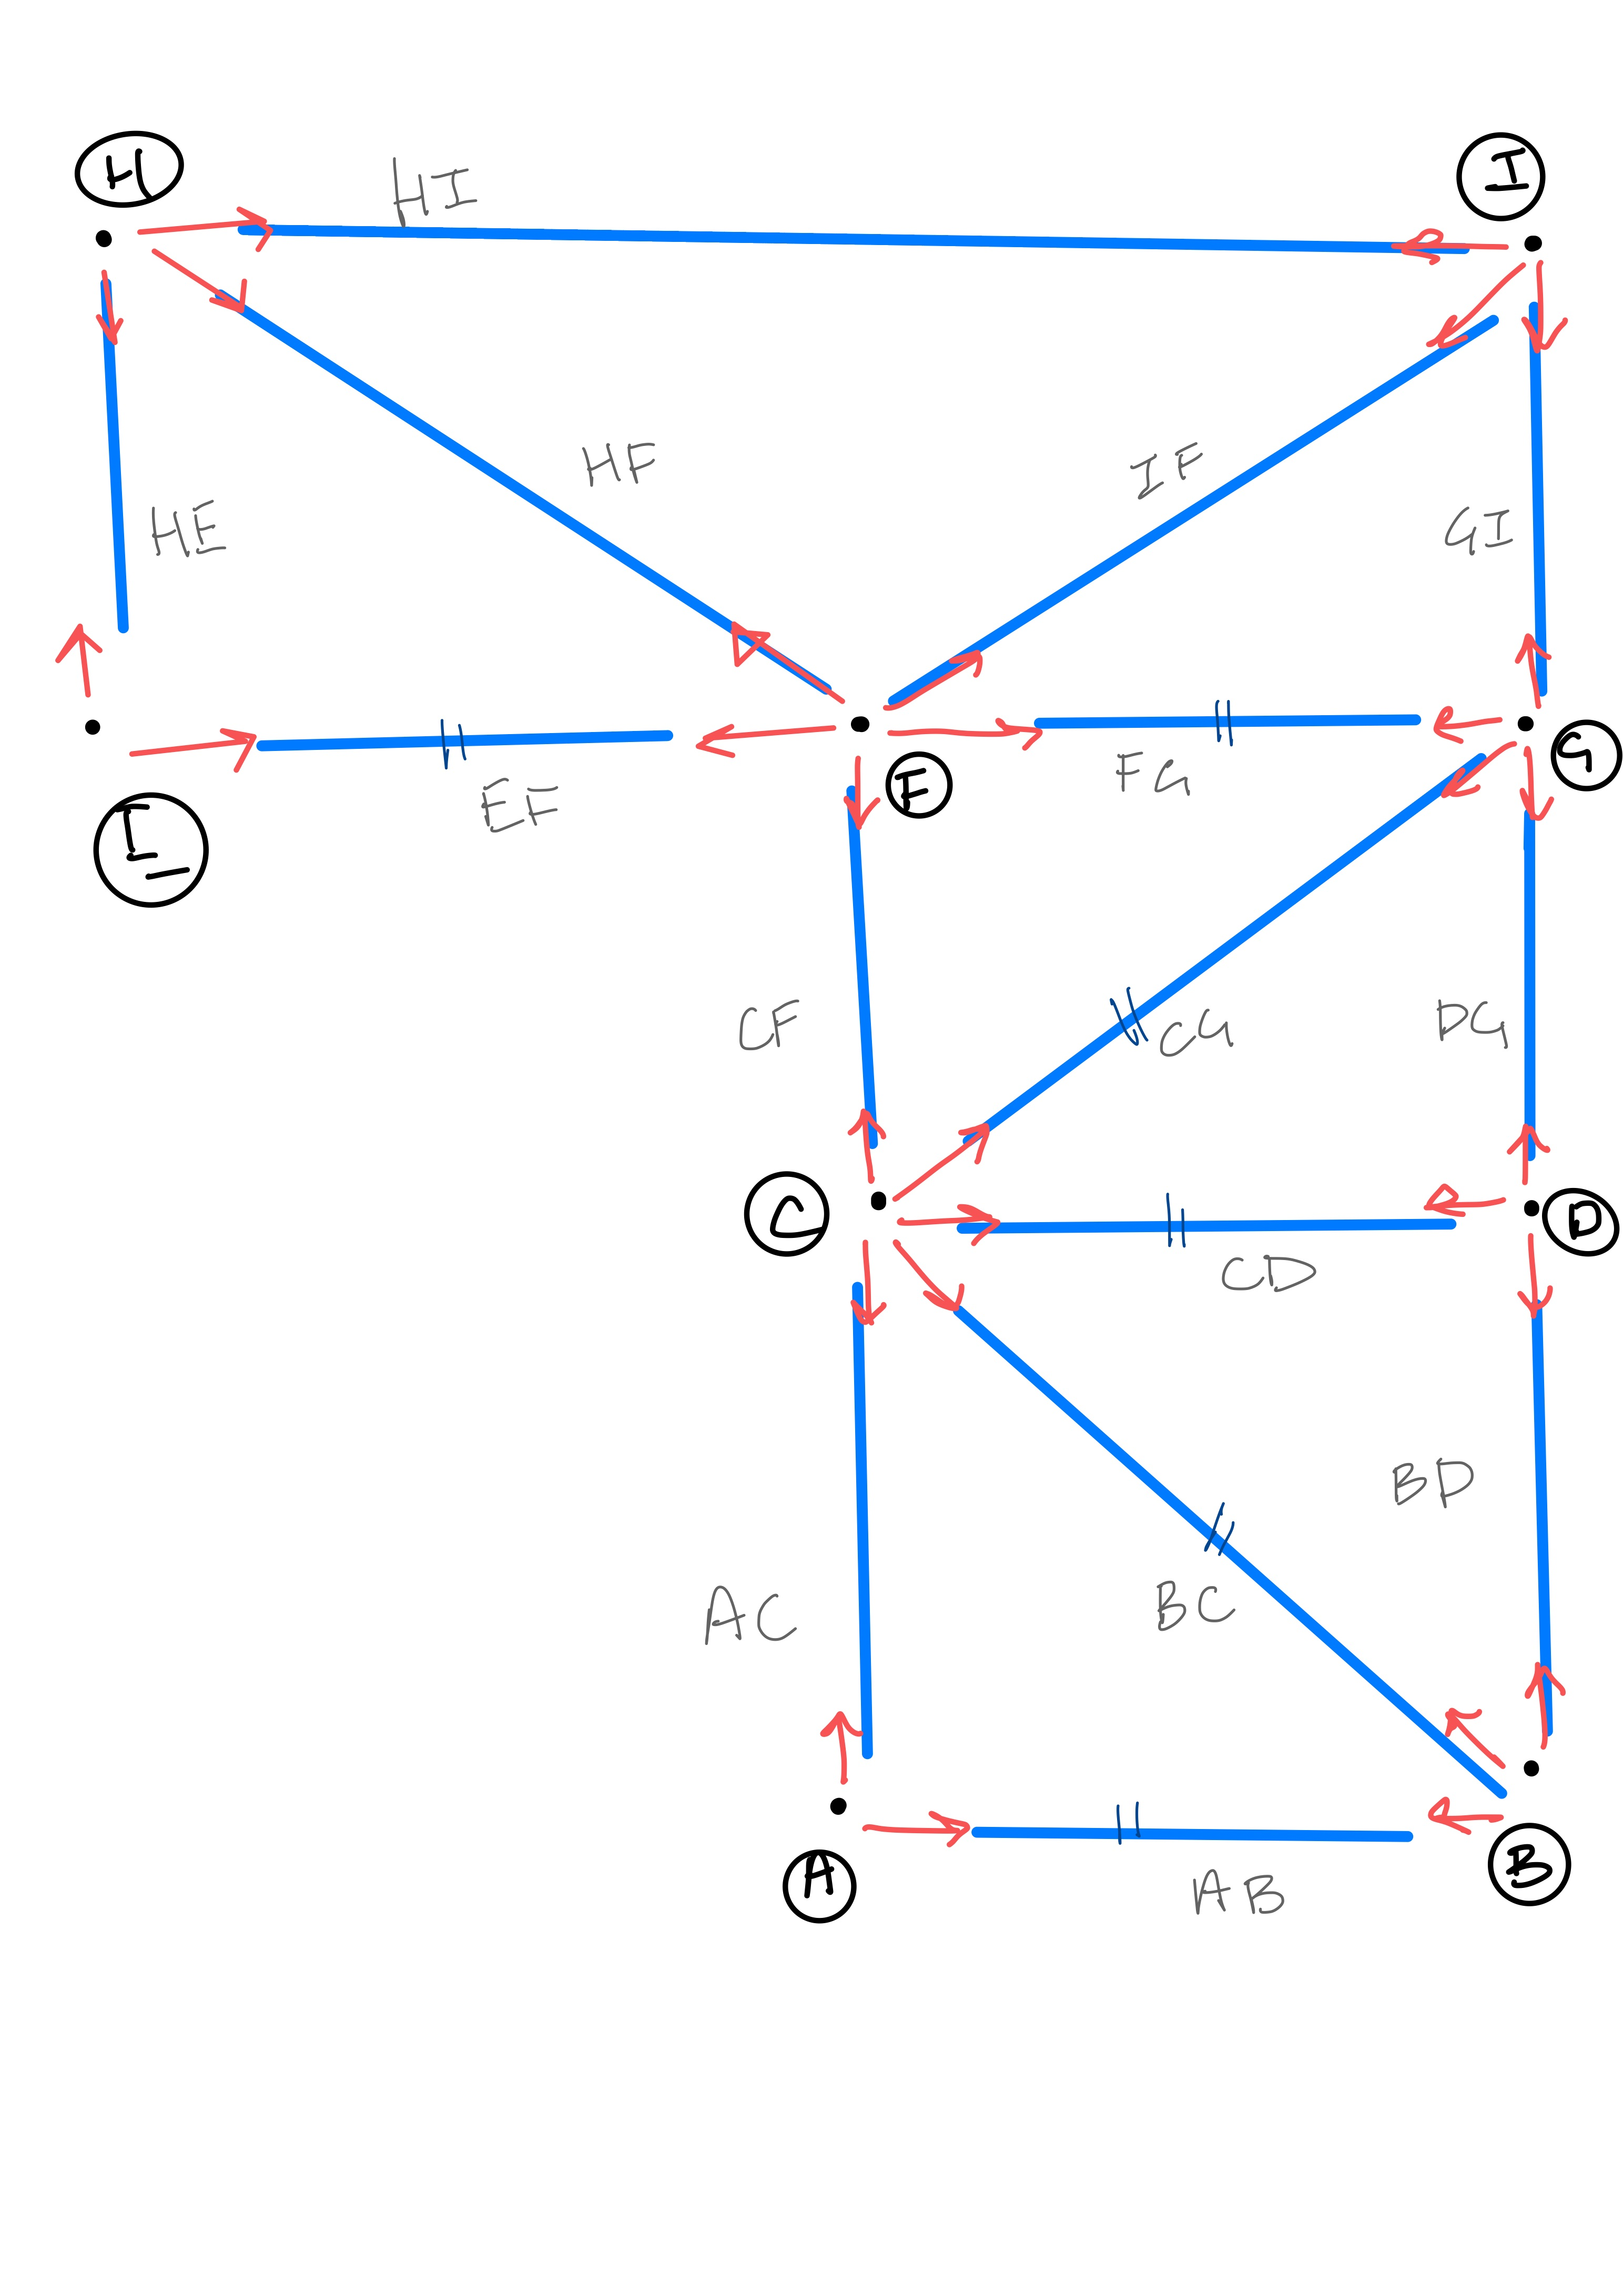
\includegraphics[width=\textwidth]{con1_fbd.jpg}
\caption{Free Body Diagram of all joints, truss system}
\end{figure}
Zero force members:
\begin{itemize}
\item EF
\item FG
\item CG
\item CD
\item BC
\item AB
\end{itemize}
\centering
\begin{tabular}{@{}cccc@{}}
\toprule
\textbf{Truss} & \textbf{Load (lb-f)} & \textbf{Force (lbf)} & \textbf{\begin{tabular}[c]{@{}c@{}}Tension ($-$)/\\ Compression ($+$)?\end{tabular}} \\ \midrule
EH & 200 & 200 & T \\
HI & 200 & 200 & T \\
IG & 133 & 133 & T \\
DG & 133 & 133 & T \\
BD & 133 & 133 & T \\
FH & -282.8 & -282.8 & C \\
FI & -240.4 & -240.4 & C \\
CF & -333 & -333 & C \\
CA & -333 & -333 & C
\end{tabular}
\subsection{Concept 1: Load Condition B}
	At $ \theta = 45 $ degrees, then we can solve for the following:
 $\frac{w}{2} = \frac{300}{2} = 150 $ lb-f. For each joint we require a free body diagram calculating each joint by method of joints.
     \subsubsection{External reactions}
$ A_x = 106.6 $ lbf, $A_y = 426.4$ lb-f. $ B_y = -319.8$ lbf.
$\overline{\mathrm{T_x}} = 150\cos(45) -0 = -75\sqrt{2} $ lb-f.
$\overline{\mathrm{T_y}} = 0 - 150\sin(45) = -75\sqrt{2} $ lb-f.
$\overline{\mathrm{T_F }} = 0 - 150\cos(45) = -75\sqrt{2}, -75\sqrt{2} = (-106.066, -106.066) $ lb-f. 
\subsubsection{Internal Forces (Compression/Tension)}
\begin{figure}
\centering
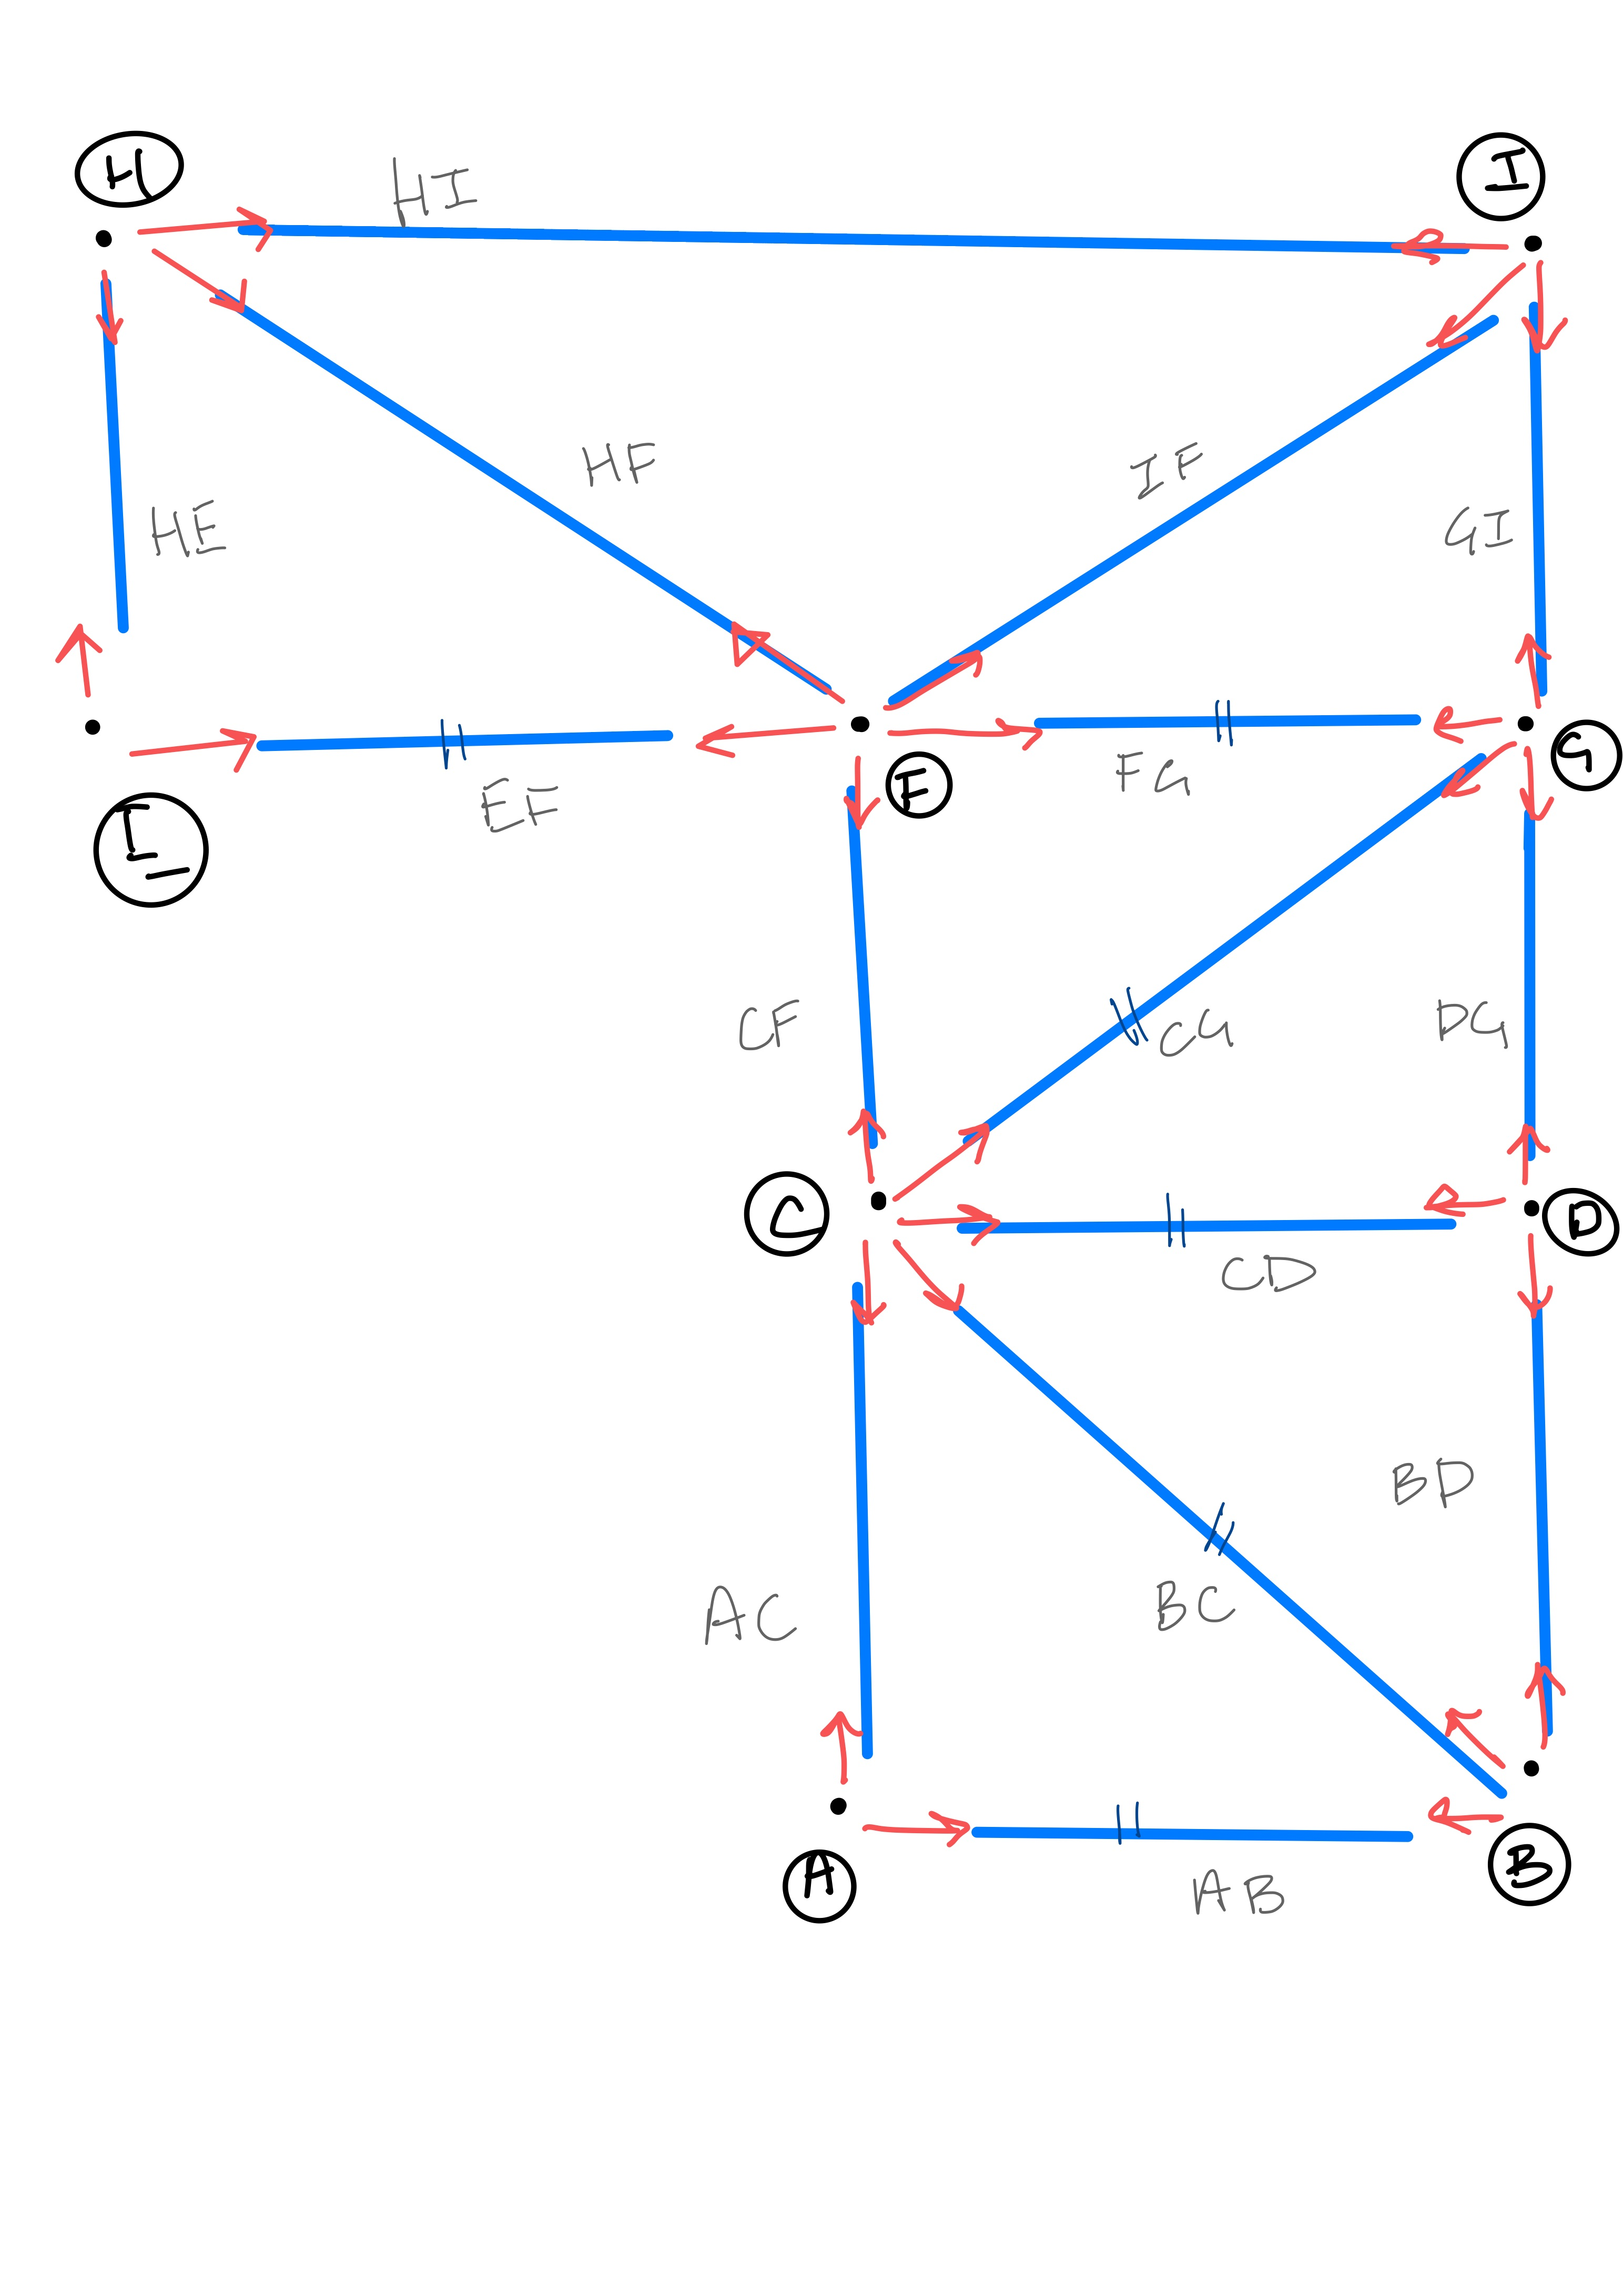
\includegraphics[width=\textwidth]{con1_fbd.jpg}
\caption{Free Body Diagram of all joints, truss system}
\end{figure}
The only zero-force member in this condition is $ \overline{\mathrm{CD}}$
\centering
\begin{tabular}{@{}cccc@{}}
\toprule
\textbf{Truss} & \textbf{Load (lb-f)} & \textbf{Force (lbf)} & \textbf{\begin{tabular}[c]{@{}c@{}}Tension ($-$)/\\ Compression ($+$)?\end{tabular}} \\ \midrule
AB & -106.6 & -106.6 & C \\
BC & 163.8 & 163.8 & T \\
AC & -426.4 & -426.4 & C \\
BD & 195.4 & 195.4 & T \\
CF & -177.7 & -177.7 & C \\
DG & 195.4 & 195.4 & T \\
CG & -163.8 & -163.8 & C \\
FG & 106.6 & 106.6 & T \\
GI & 71.07 & 71.07 & T \\
HI & 106.6 & 106.6 & T \\
HE & 106.6 & 106.6 & T \\
EF & 106.6 & 106.6 & T \\
HF & -150.8 & -150.8 & C \\
FI & -128.1 & -128. & C
\end{tabular}
\subsection{Concept 2: Load Condition A}
	At $ \theta = 0 $ degrees, then we can solve for the following: $\frac{w}{2} = \frac{400}{2} = -200 $ lb-f. For each joint we require a free body diagram calculating each joint by method of joints.
    In this structure, the trusses have joints that connect members that are aligned along the same line. Therefore, the conditions for joints being under the zero force members is satisfied on the 2D representation of the frame.
    Identifying the zero force members:
\begin{itemize}
\item EF
\item FG
\item CD
\item BC
\item AB
\item CG
\end{itemize}
    \subsubsection{External reactions}
$\Sigma F_x = 0$, $A_y = + 333$ lbf, $Ax = + 0 $ lbf
$\Sigma F_y = 0; B_y = -133 \longleftarrow \frac{W}{4} = \frac{533}{4} = 133 $ lbf.
    \subsubsection{Internal Forces (Tension/Compression)}
\begin{figure}
\centering
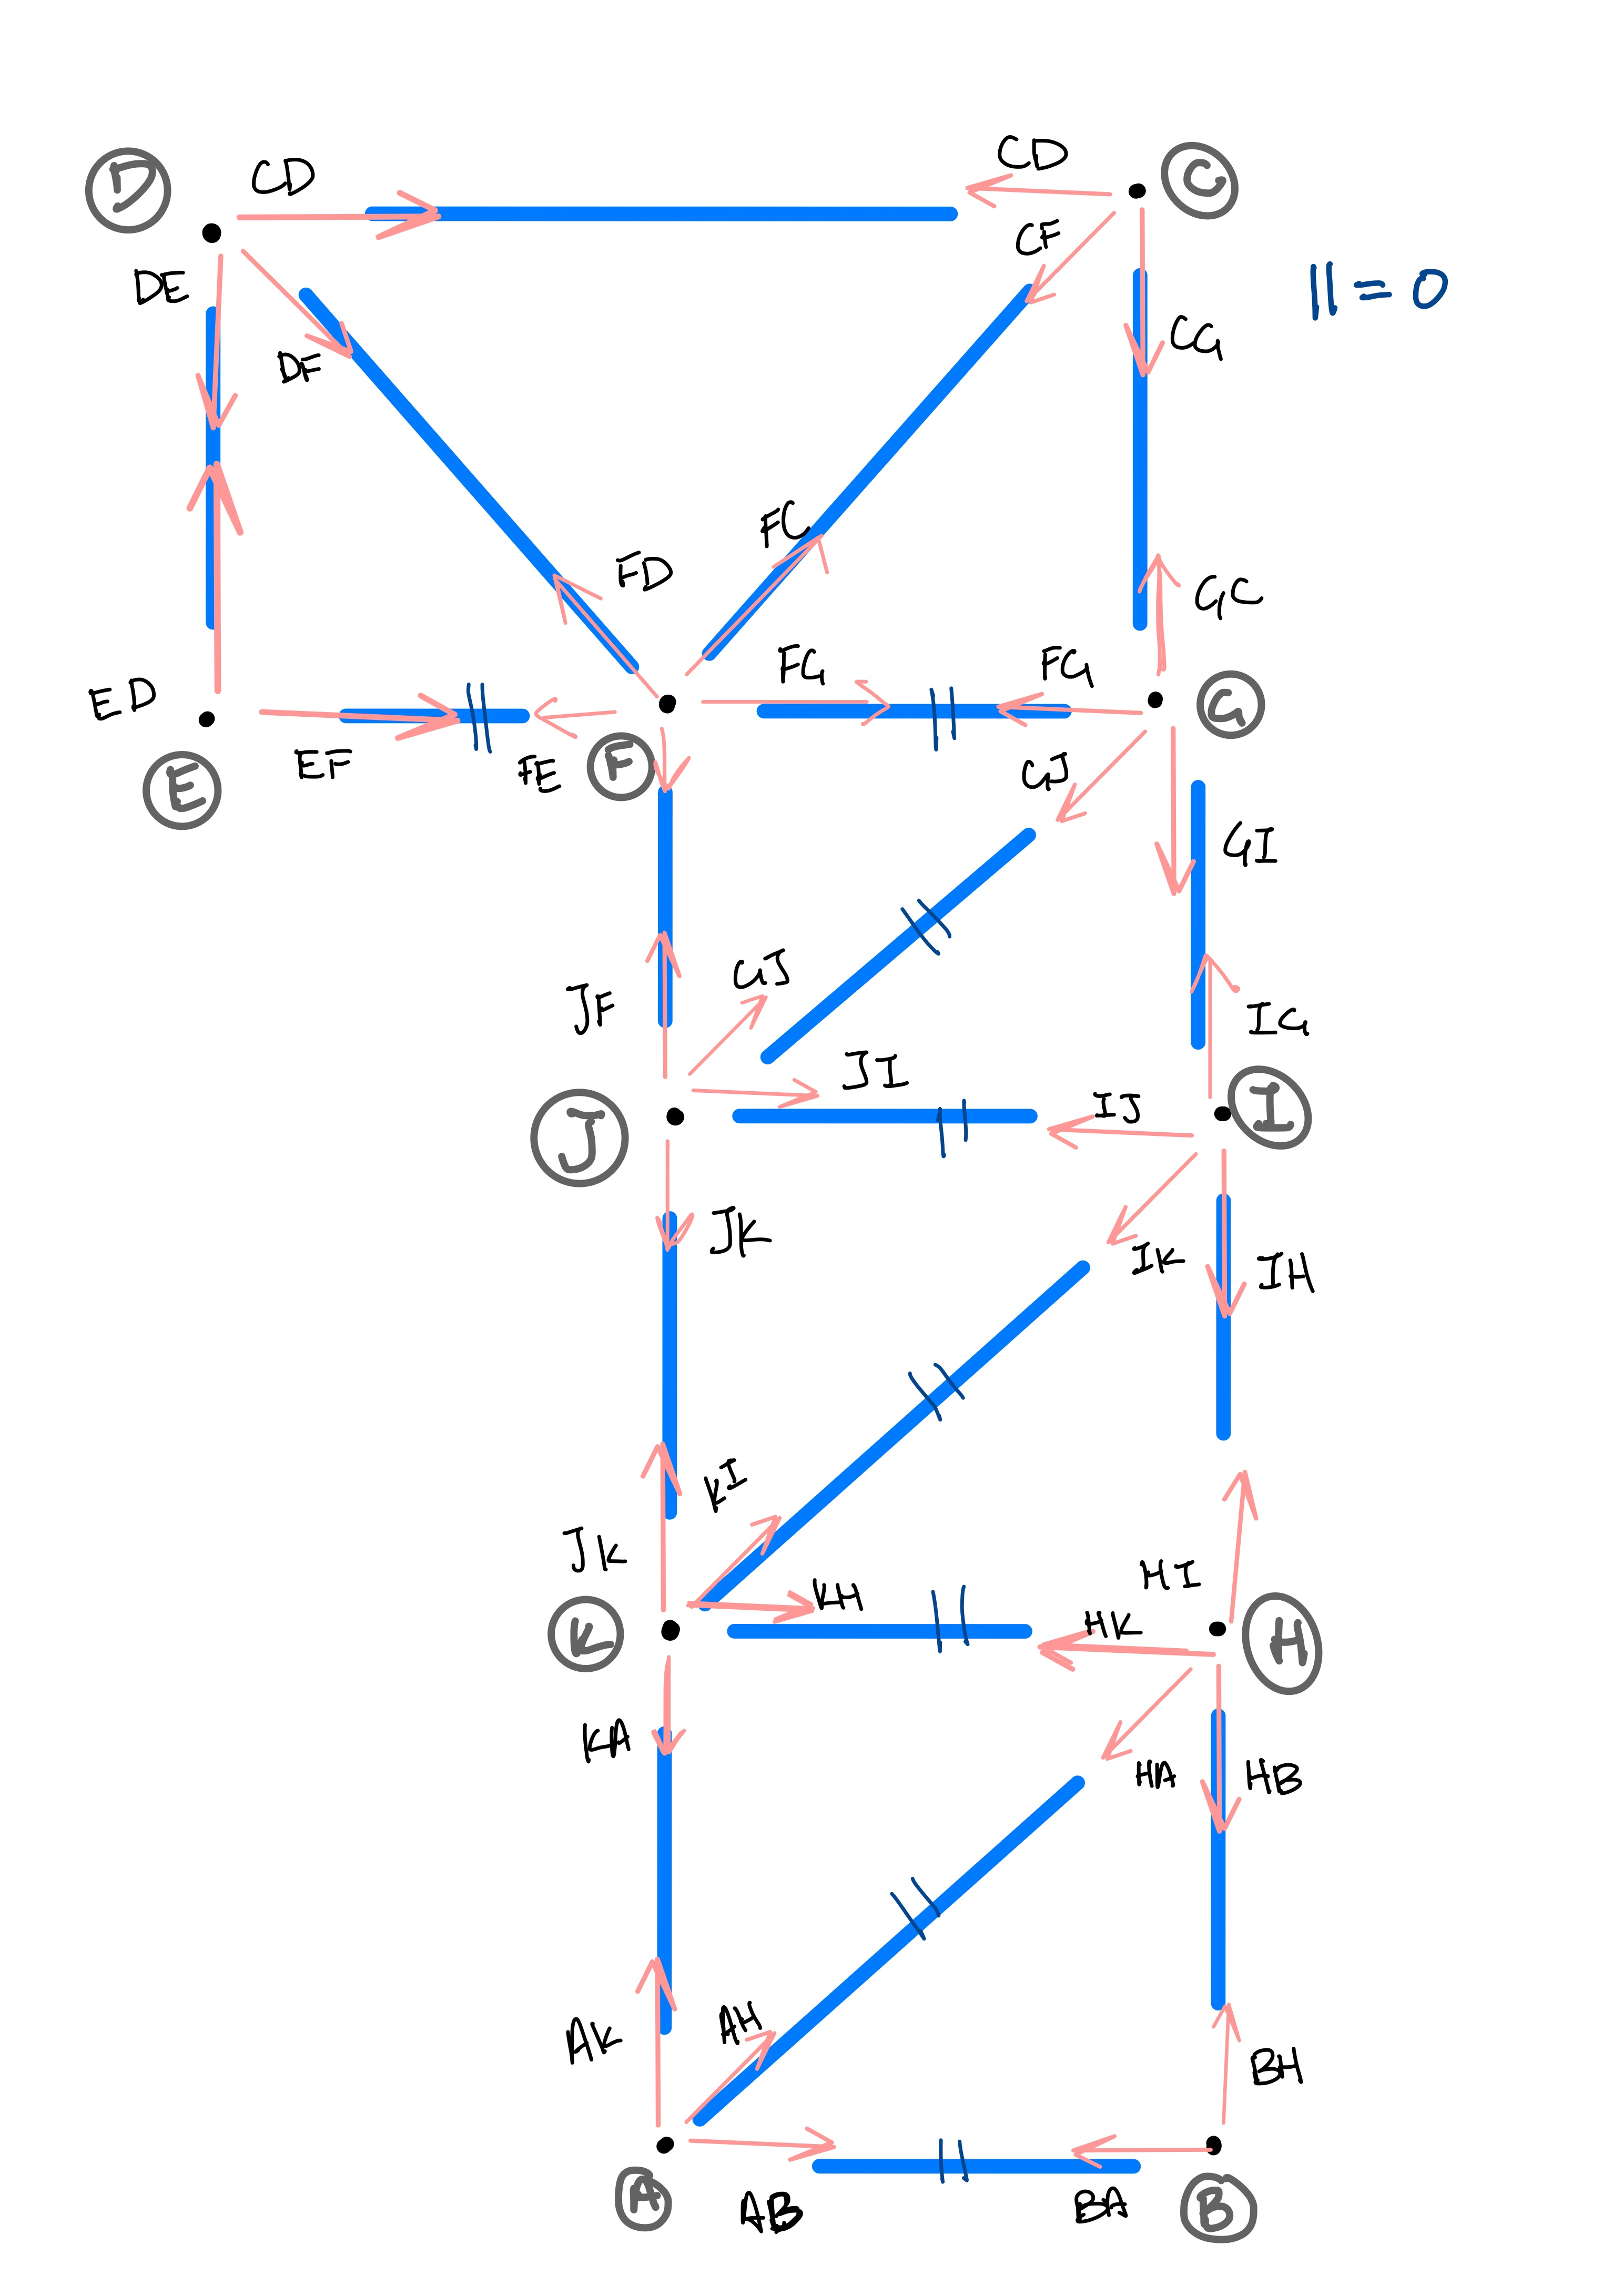
\includegraphics[width=\textwidth]{con2_fbd.jpg}
\caption{Free Body Diagram of all joints, truss system}
\end{figure}
$ \Sigma F_x = 0 $ ; $ \overline{\mathrm AB} = 0$;
Between $\overline{\mathrm BC} \| \overline{\mathrm CF} \| \overline{\mathrm FG} \| \overline{\mathrm AD} \| \overline{\mathrm DE} \| \overline{\mathrm EI}$ are all at a height of $28$ inches. $\overline{\mathrm KJ} \| \overline{\mathrm HG} = 24 $ inches. By solving the right triangle inequality of each truss, for example, taking the first triangle at the bottom of half of $ \square ABHK$ : 
$$ 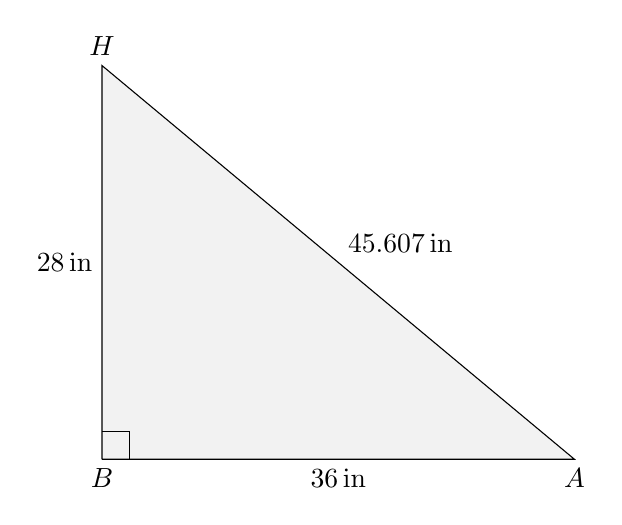
\begin{tikzpicture}
% Draw the triangle
        \draw[fill=gray!10]  (0, 0) coordinate (A) 
        -- node[left] {$28$\,in} (0,5) coordinate (C) 
        -- node[above right] {$45.607$\,in} (6,0) coordinate (B)  -- node[below] {$36$\,in}  (0, 0);
       \draw (0,10pt) -- ++(10pt,0) -- ++(0,-10pt);
% Draw nodes
        \node at (A)[anchor=north] {$B$};
        \node at (B)[anchor=north] {$A$};
        \node at (C)[anchor=south] {$H$};
      \end{tikzpicture} $$Zero-force members identified:
$$ \overline{\mathrm AB} \| \overline{\mathrm AH } \| \overline{\mathrm KH } \| \overline{\mathrm KI} \| \overline{\mathrm FG} \| \overline{\mathrm GJ} \| \overline{\mathrm EF}$$
Using this information, theta is calculated as such: $ \theta = \arctan( \frac{28}{36}) = 37.87 ^{\circ} $. $ \Sigma F_x = 0 $ which gives us the ability to calculate from $ AC = 0 \longrightarrow AB - AC \cos(37.87) = 0$. 
For $ \Sigma F_y = 0 $, $AD = 28$ inches, then we can calculate from previously solved unknowns of external force $-133 \downarrow = AD $ against the external force on pin $A = +467 \uparrow $ gives the solution to $AD$ as $AD = 467-133 = 334$ lb-f. As I've proven a bit, I will use matrices for the rest of the representations:
 \centering
\begin{tabular}{@{}cccc@{}}
\toprule
\textbf{Truss} & \textbf{Load (lb-f)} & \textbf{Force (lbf)} & \textbf{\begin{tabular}[c]{@{}c@{}}Tension ($-$)/\\ Compression ($+$)?\end{tabular}} \\ \midrule
BH & 133.3 & 133.3 & T \\
AK & -333.3 & -333.3 & C \\
HI & 133 & 133 & T \\
IG & 133 & 133 & T \\
GC & 133 & 133 & T \\
CD & 200 & 200 & T \\
DE & 200 & 200 & T \\
DF & -282.8 & -282.8 & C \\
FG & -240.4 & -240.4 & C \\
JK & -333 & -333 & C \\
JF & -333 & -333 & C \\ \bottomrule
\end{tabular}
\subsection{Concept 2: Load Condition B}
	At $ \theta = 45 $ degrees, then we can solve for the following: $\frac{w}{2} = \frac{300}{2} = 150 $ lb-f. For each joint we require a free body diagram calculating each joint by method of joints. Zero force member this time is only $\overline{\mathrm{AB}}$.
\subsubsection{External Reactions}
$\Sigma F_x = 0$, $A_y = + 424.4 lbf, $Ax = + 106.1 lbf
$\Sigma F_y = 0; B_y =-318.3 $ lbf.    
$\overline{\mathrm{T_x}} = 150\cos(45) -0 = -75\sqrt{2} $ lb-f.
$\overline{\mathrm{T_y}} = 0 - 150\sin(45) = -75\sqrt{2} $ lb-f.
$\overline{\mathrm{T_F }} = 0 - 150\cos(45) = -75\sqrt{2}, -75\sqrt{2} = (-106.066, -106.066) $ lb-f. 
\subsubsection{Internal Forces}
\begin{figure}
\centering
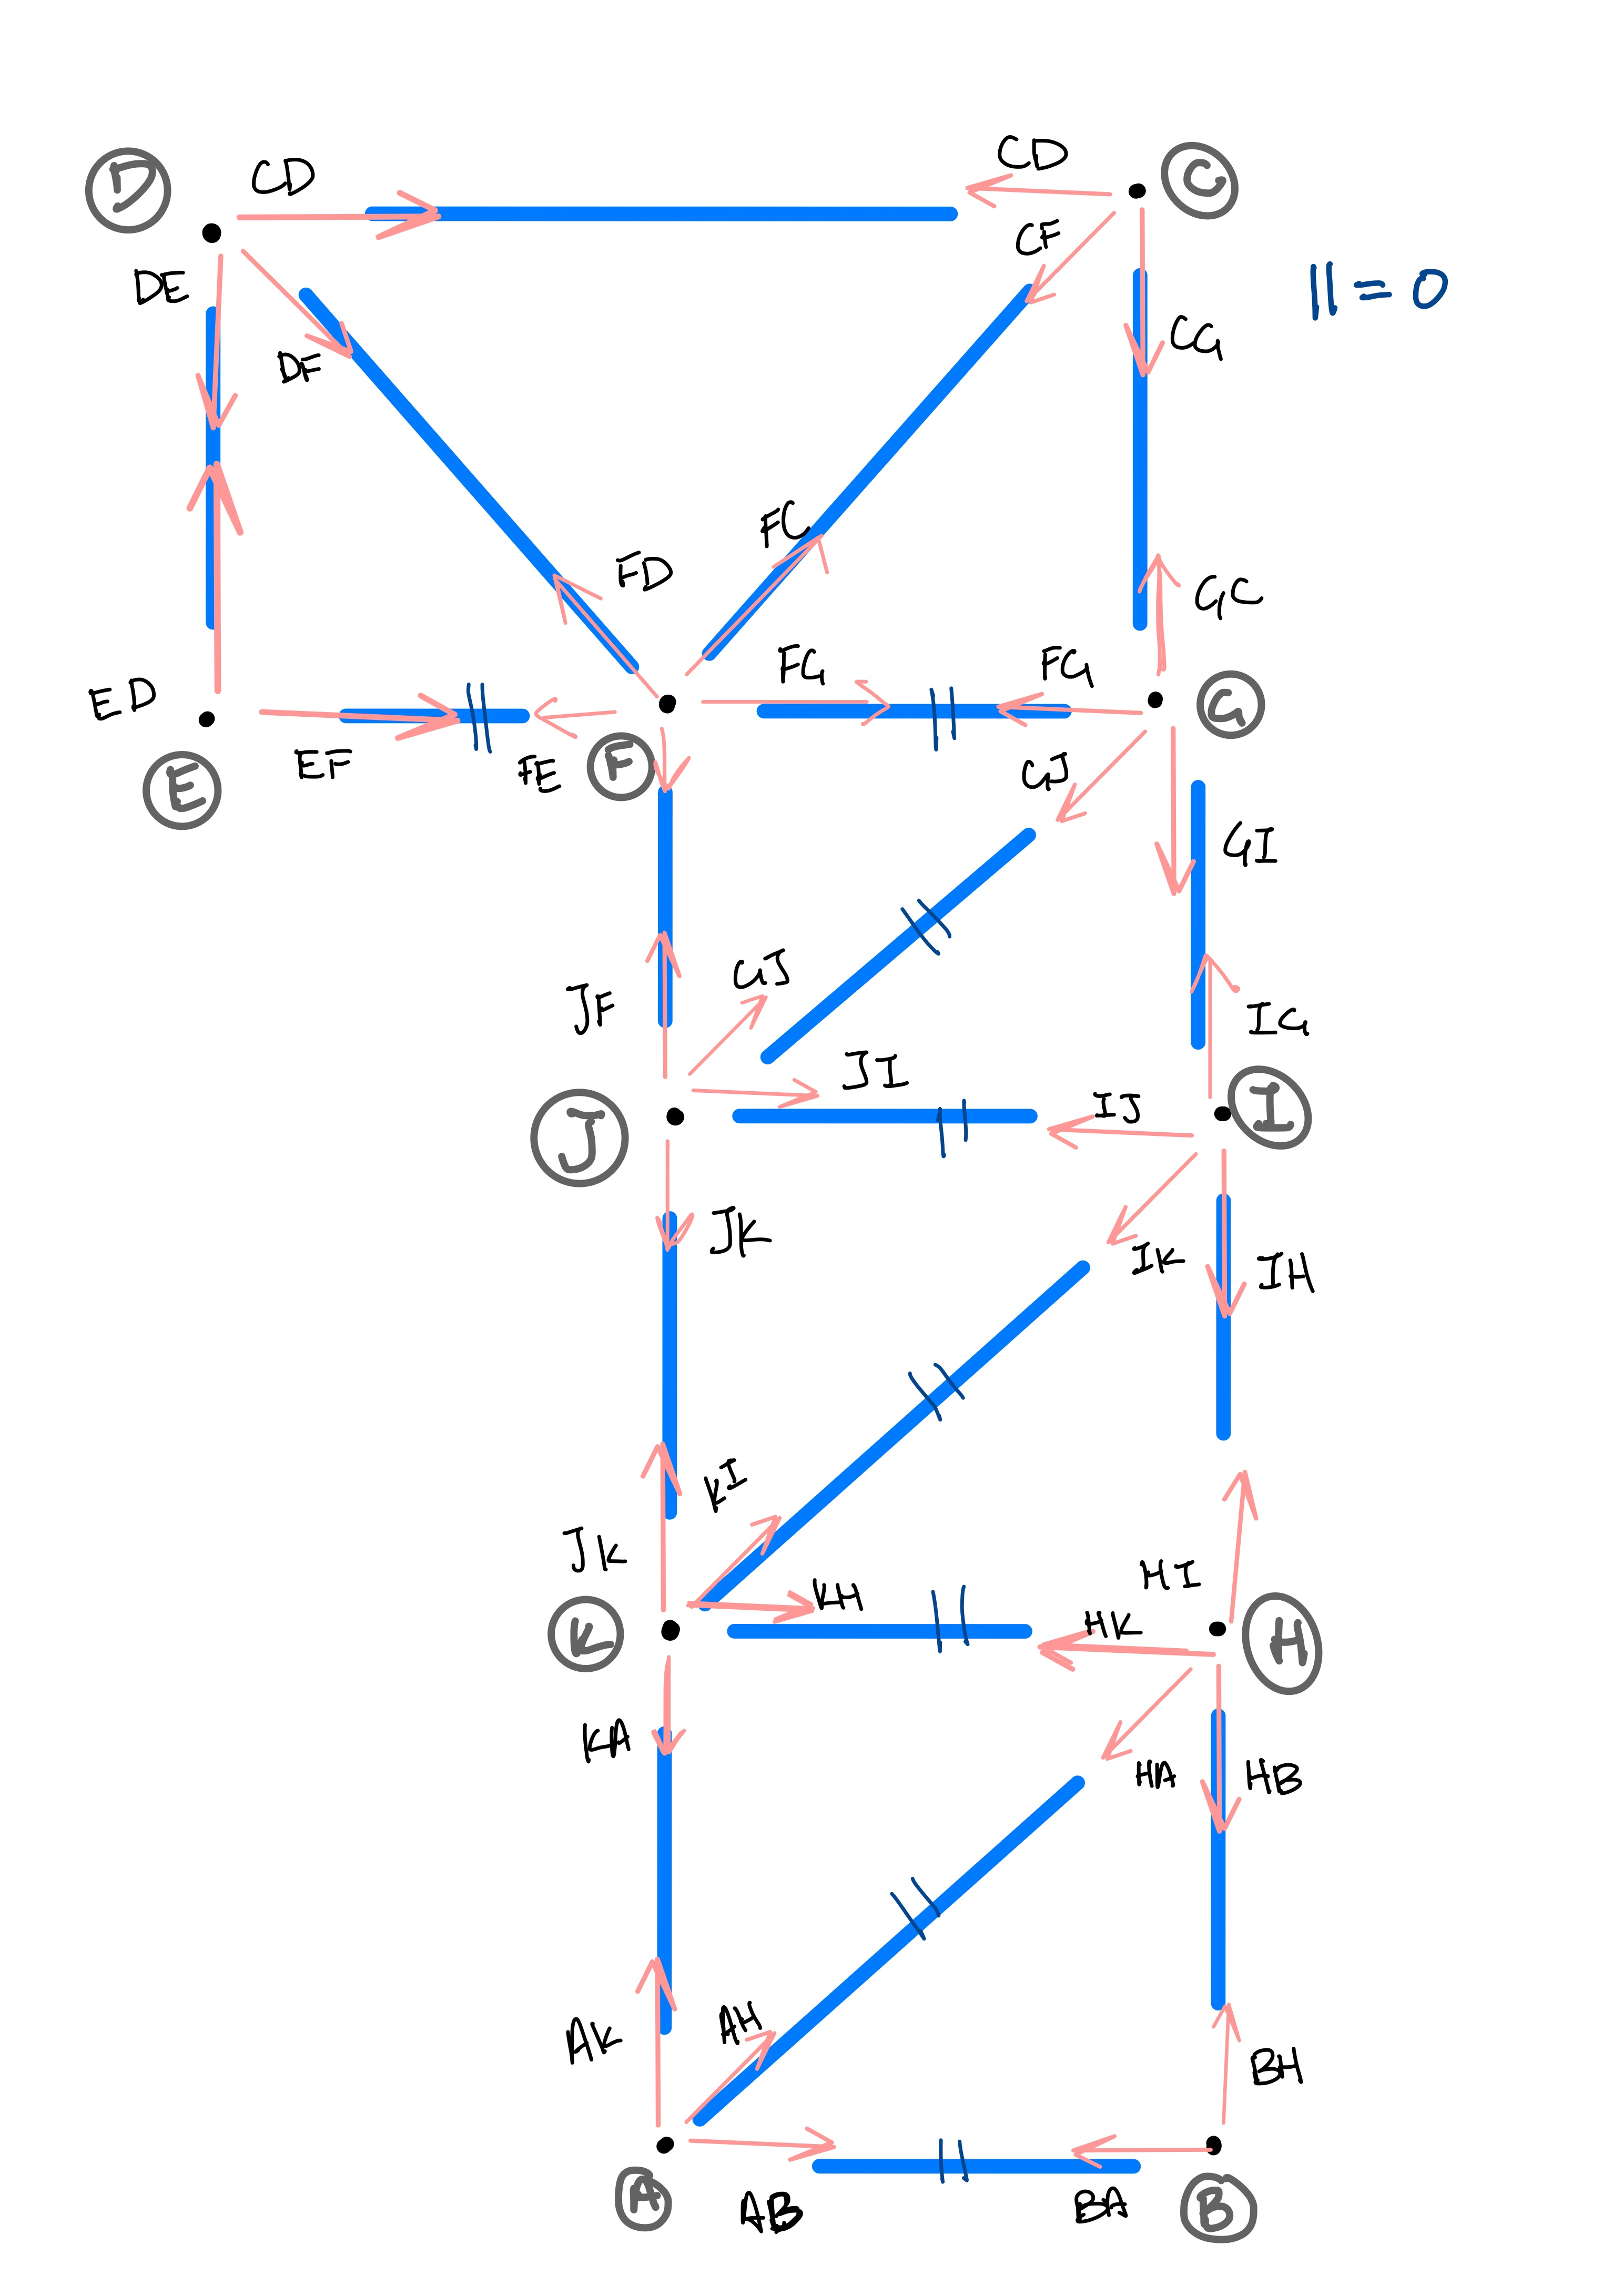
\includegraphics[width=\textwidth]{con2_fbd.jpg}
\caption{Free Body Diagram of all joints, truss system}
\end{figure}
 \centering
\begin{tabular}{@{}cccc@{}}
\toprule
\textbf{Truss} & \textbf{Load (lb-f)} & \textbf{Force (lbf)} & \textbf{\begin{tabular}[c]{@{}c@{}}Tension ($-$)/\\ Compression ($+$)?\end{tabular}} \\ \midrule
Node & Load (lb-f) & Force (lb-f) & Tensi \\
AH & -134.4 & -134.4 & C \\
BH & 318.3 & 318.3 & T \\
HK & 106.1 & 106.1 & T \\
AK & -341.9 & -341.9 & C \\
IH & 235.8 & 235.8 & T \\
JK & -259.4 & -259.4 & C \\
IK & -134.4 & -134.4 & C \\
JI & 106.1 & 106.1 & T \\
JF & -176.8 & -176.8 & C \\
GI & 153.3 & 153.3 & T \\
GJ & -134.4 & -134.4 & C \\
FG & 106.1 & 106.1 & T \\
CG & 70.73 & 70.73 & T \\
CD & 106.1 & 106.1 & T \\
DE & 106.1 & 106.1 & T \\
EF & 106.1 & 106.1 & T \\
DF & -150.0 & -150.0 & C \\
FC & -127.5 & -127.5 & C
\end{tabular}
\subsection{Concept 3: Load Condition A}
	At $ \theta = 0 $ degrees, then we can solve for the following: $\frac{w}{2} = \frac{400}{2} = -200 $ lb-f. For each joint we require a free body diagram calculating each joint by method of joints.
        \subsubsection{External reactions}
$\Sigma F_x = 0$, $A_y = + 424.4 lbf, $Ax = + 106.1 lbf
$\Sigma F_y = 0; B_y =-318.3 $ lbf.    
\subsubsection{Internal Forces (Compression/Tension)}
\begin{figure}
\centering
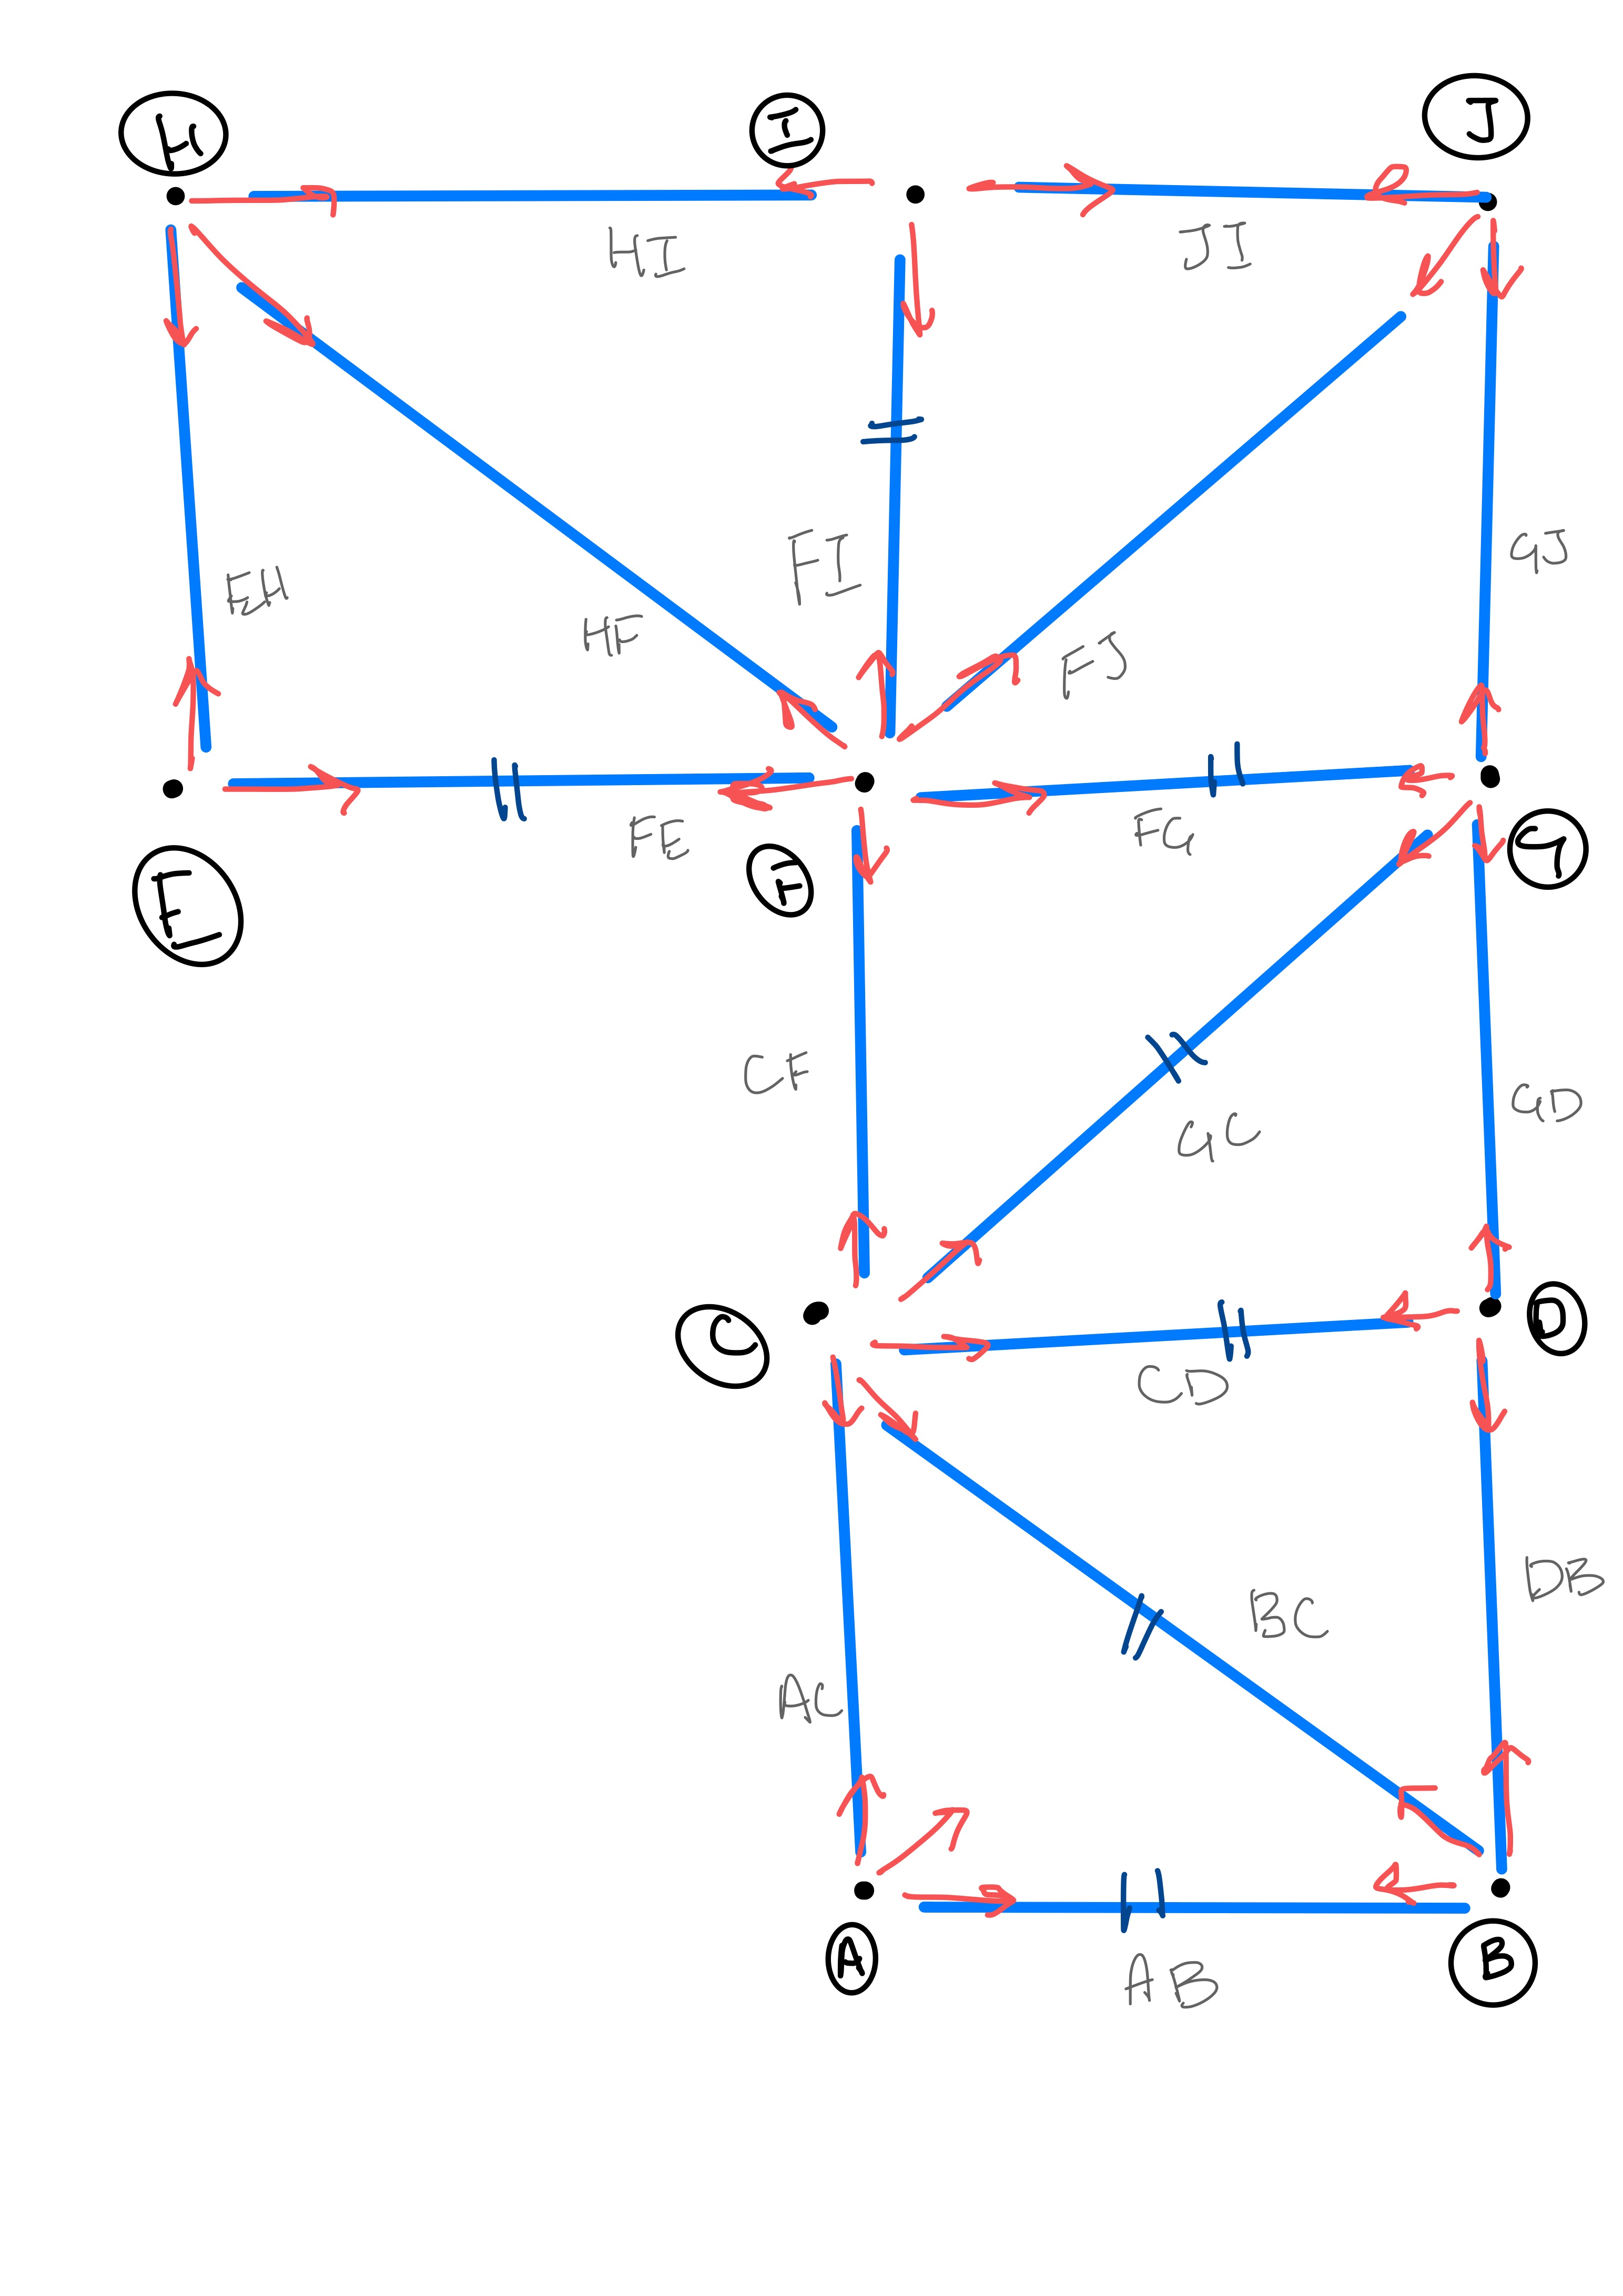
\includegraphics[width=\textwidth]{con3_fbd.jpg}
\caption{Free Body Diagram of all joints, truss system}
\end{figure}
Zero-force members:
\begin{itemize}
\item EF
\item FG
\item CG
\item CD
\item BC
\item AB
\item FI
\end{itemize}

\centering
\begin{tabular}{@{}cccc@{}}
\toprule
\textbf{Truss} & \textbf{Load (lb-f)} & \textbf{Force (lbf)} & \textbf{\begin{tabular}[c]{@{}c@{}}Tension ($-$)/\\ Compression ($+$)?\end{tabular}} \\ \midrule
HE & 200 & 200 & T \\
HI & 200 & 200 & T \\
IJ & 200 & 200 & T \\
JG & 133 & 133 & T \\
GD & 133 & 133 & T \\
BD & 133 & 133 & T \\
AC & -333 & -333 & C \\
CF & -333 & -333 & C \\
\end{tabular}
\subsection{Concept 3: Load Condition B}
	At $ \theta = 45 $ degrees, then we can solve for the following: $\frac{w}{2} = \frac{300}{2} = 150 $ lb-f. For each joint we require a free body diagram calculating each joint by method of joints.
     \subsubsection{External reactions}
$\Sigma F_x = 0$, $A_y = + 424.4 lbf, $Ax = + 106.1 lbf
$\Sigma F_y = 0; B_y =-318.3 $ lbf.    
$\overline{\mathrm{T_x}} = 150\cos(45) -0 = -75\sqrt{2} $ lb-f.
$\overline{\mathrm{T_y}} = 0 - 150\sin(45) = -75\sqrt{2} $ lb-f.
$\overline{\mathrm{T_F }} = 0 - 150\cos(45) = -75\sqrt{2}, -75\sqrt{2} = (-106.066, -106.066) $ lb-f. 
\subsubsection{Internal Forces (Compression/Tension)}
\begin{figure}
\centering
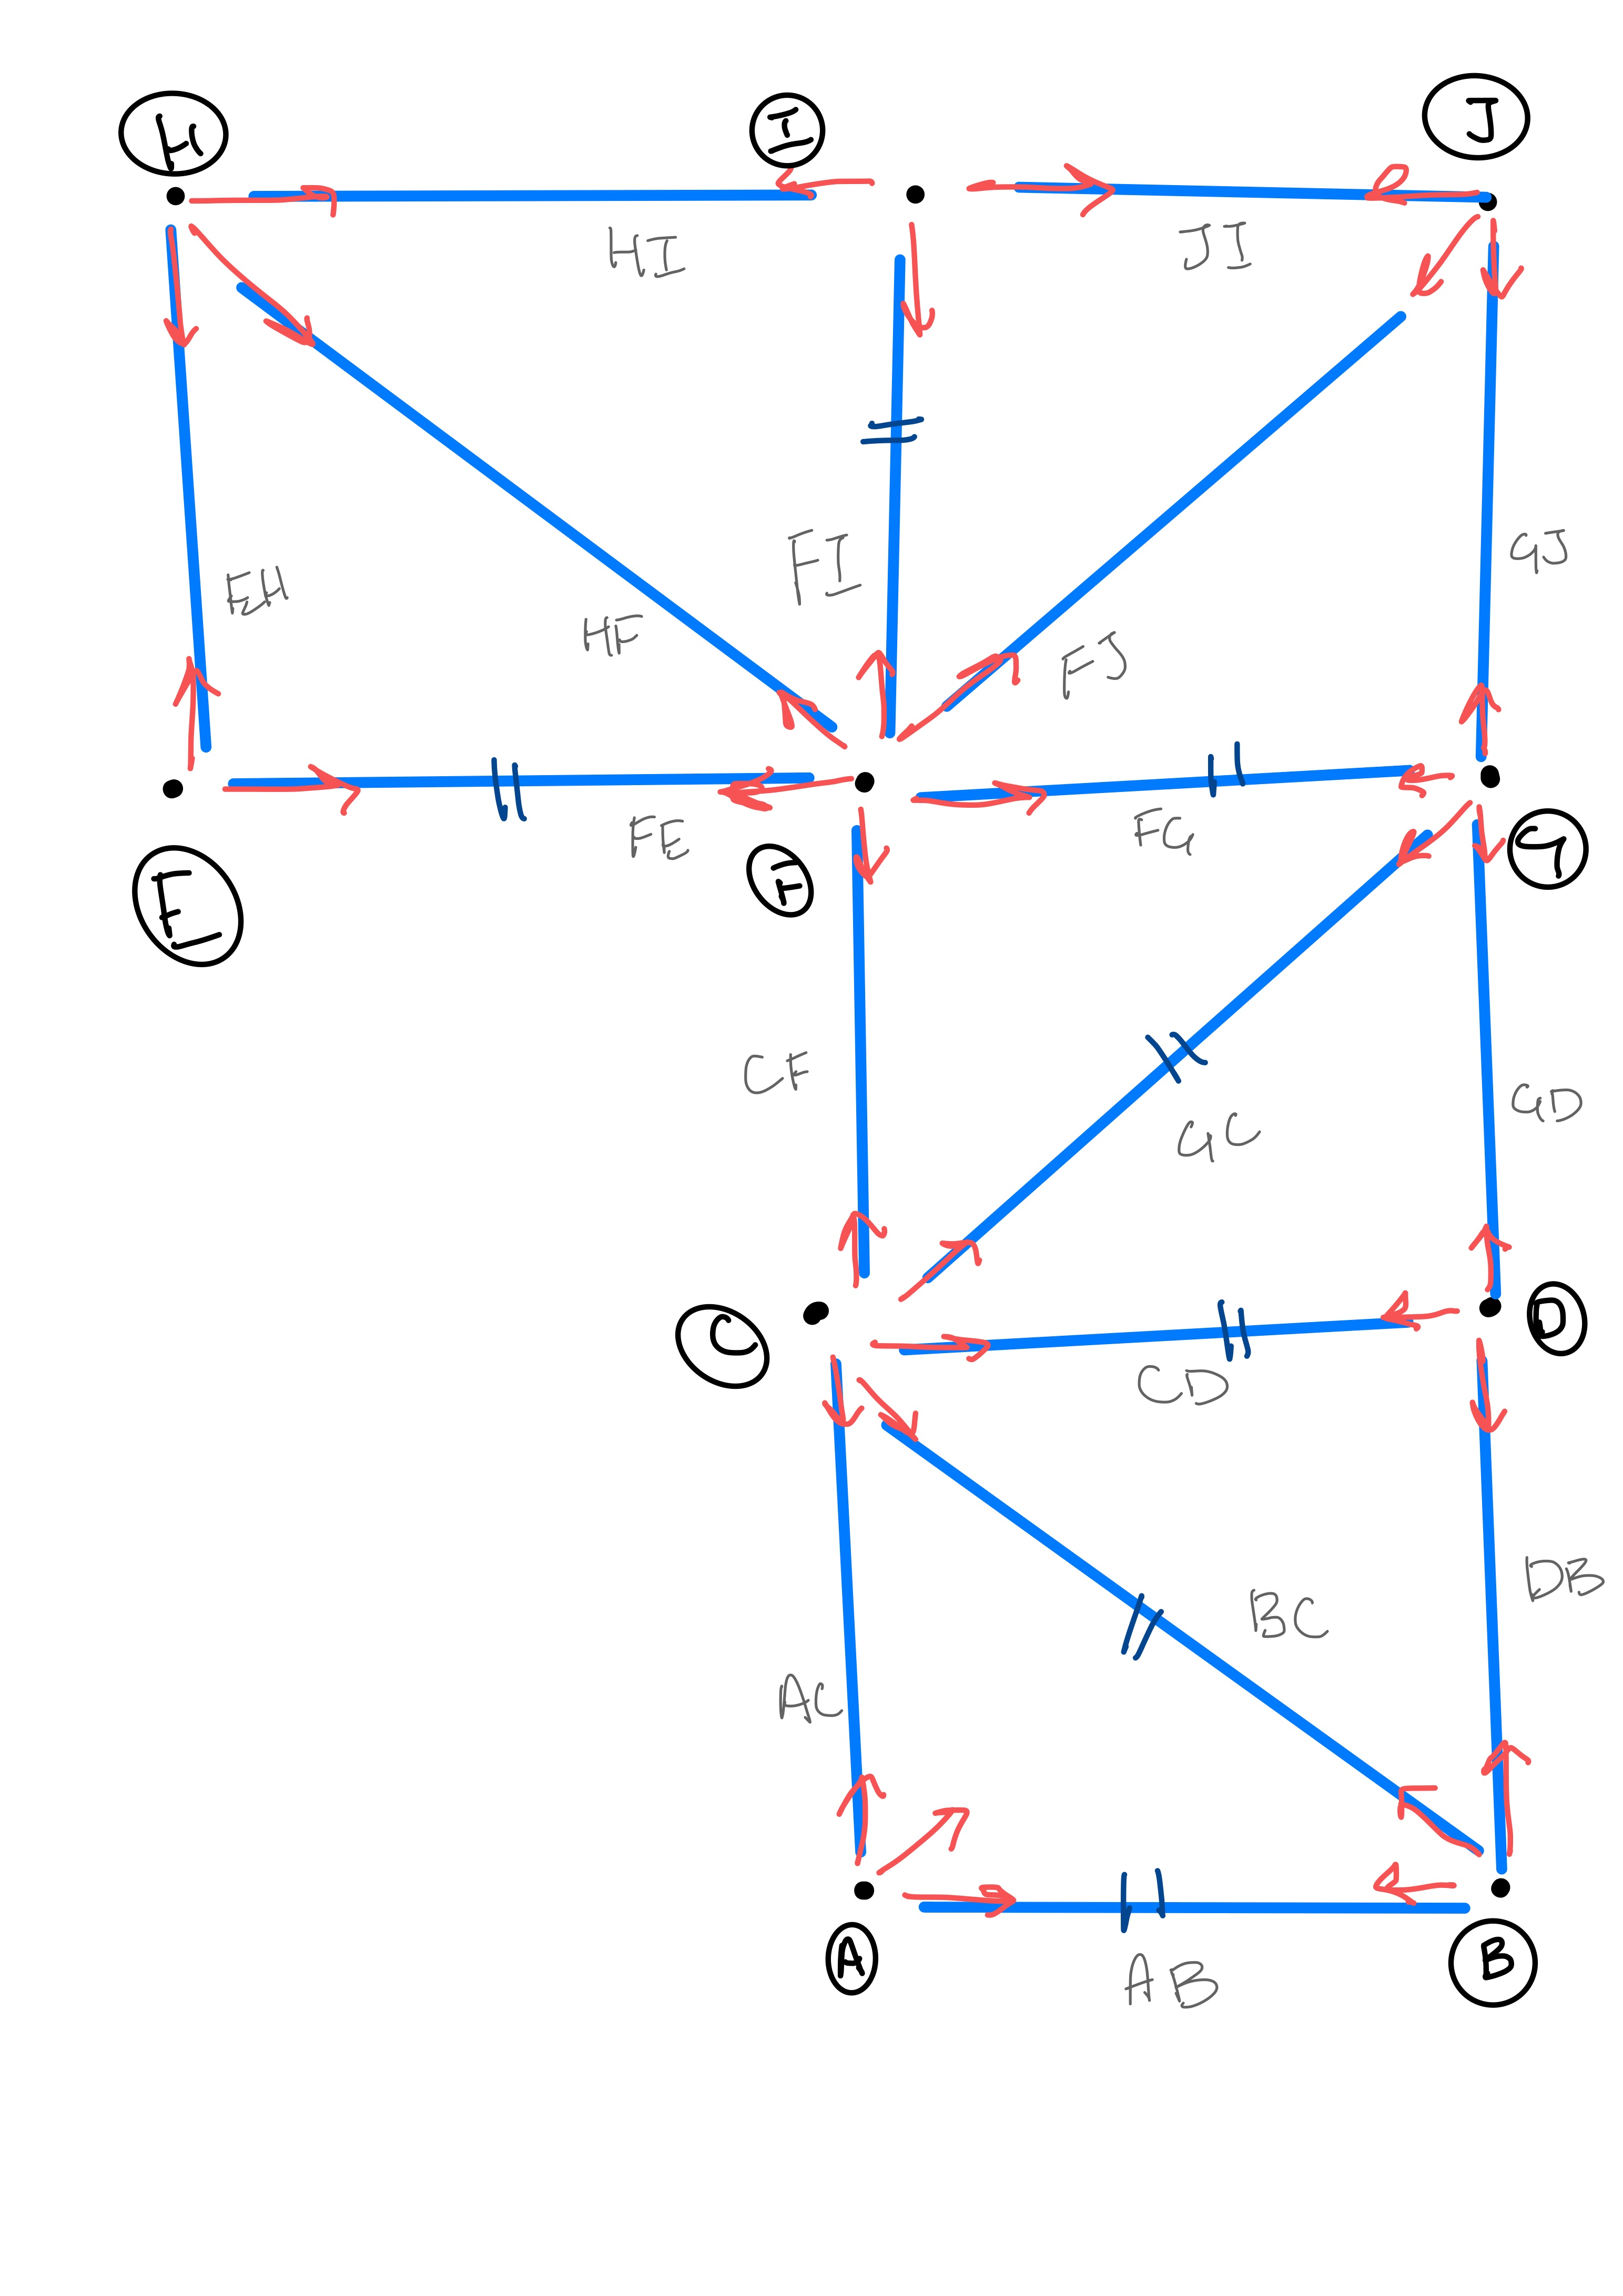
\includegraphics[width=\textwidth]{con3_fbd.jpg}
\caption{Free Body Diagram of all joints, truss system}
\end{figure}
Zero-force members:
\begin{itemize}
\item CD
\item FI
\end{itemize}
\centering
\begin{tabular}{@{}cccc@{}}
\toprule
\textbf{Truss} & \textbf{Load (lb-f)} & \textbf{Force (lbf)} & \textbf{\begin{tabular}[c]{@{}c@{}}Tension ($-$)/\\ Compression ($+$)?\end{tabular}} \\ \midrule
AB & -106 & -106 & C \\
BD & 194.33 & 194.33 & T \\
BC & 162.88 & 162.88 & T \\
AC & -424 & -424 & C \\
CF & -176.67 & -176.67 & C \\
CG & -162.88 & -162.88 & C \\
GD & 194.33 & 194.33 & T \\
FG & 106 & 106 & T \\
GJ & 70.67 & 70.67 & T \\
JI & 106 & 106 & T \\
HI & 106 & 106 & T \\
HE & 106 & 106 & T \\
EF & 106 & 106 & T \\
HF & -149.91 & -149.91 & C \\
FJ & -127.4 & -127.4 & C \\
\end{tabular}
\chapter{Conclusions}
\section{Design Concept Selection}
	Based on the analysis and the engineering requirements, out of the three preliminary design concepts that should be considered as a potential solution to this structural design problem I consider the third conceptual design structure explored as the a potential solution.
The truss design that does not exceed the truss member load ratings in any given member and has the least total length should be selected. Also, taking into consideration the shear/force displacement, although there is bending/distortion, it is, compared to the three design concepts, the least displaced. I believe the concept can be modified to meet the design requirements with more time. Unfortunately, the little time spent on this design project was what hindered the accuracy of this solution.
\subsection{Feasibility of the Design Concept}
	The widespread unavailability and difficult to assemble home gym products make the solution to the design of a labile suspension trainer a medical necessity as well as a future for the better development of people, using the concepts of mechanics/statics, it is possible to solve anything with trusses. Trusses are a tried and true method of finding well designed structures. By testing the system of trusses with frames by solving for the unknowns, the solution to the design concepts are more obvious. The feasibility of the portability is still unclear, due to the fact that the most targeted consumer is those with Traumatic Brain Injury (TBI), elderly, and those affected with PTSD. Unfortunately, this is a barrier to building that it does not have a simple way to manufacture and set up in a way with trusses. Manufacturing and building and the concepts are easy, however, the assembly, set up, installation, explanation, and other factors among the production of concept is what will set this product back. Not only that, but in the business side of things, it brings up concerns such as price. I do not see feasibility of this being sold in a completely safe way, even if the solution is found, because there is no good way to teach basic physics to prevent harm to the average person or especially those who require accommodations to bridge the gap to understand this independently.
\chapter{Recommendations}
	As the demand for a suspension trainer system that leverages the users' weight and body against the gravity to develop core stability increased after the invention of labile suspension anchoring systems for physical development, so did the methods of creating portable, home systems that were created by home enthusiasts. I would recommend the concept of portable labile suspension trainers such as the ones that leverage the user's body against the gravity of a structure. The method of weight and gravity against a structure against a single anchor point is not beaten and is still being studied. However, a truly efficient solution is hard to reach and requires much more time and studies.